\documentclass[12pt]{article}

% 加载必要的宏包，避免重复加载
\usepackage{amsmath,amsthm,amsfonts,amscd,amssymb,bm,eucal,latexsym,mathrsfs,esint}
\usepackage{tabularx,booktabs,caption,subcaption,xcolor}
\usepackage{longtable,pdflscape,threeparttable,setspace}
\usepackage{appendix,array,hyperref,listings,makecell}
\usepackage[all,cmtip]{xy}
\usepackage{geometry,graphicx}
\usepackage[most]{tcolorbox}
\usepackage{fancyhdr}
\usepackage[figuresright]{rotating} %用于旋转表格
\usepackage[fontset=none]{ctex} % 用于支持中文，不使用预设字体集

% 设置字体
\setCJKmainfont[ItalicFont={Source Han Serif SC}, SlantedFont={Source Han Serif SC}]{Source Han Serif SC}
\setCJKsansfont[ItalicFont={Source Han Serif SC}, SlantedFont={Source Han Serif SC}]{Source Han Serif SC}
\setCJKmonofont[ItalicFont={Source Han Serif SC}, SlantedFont={Source Han Serif SC}]{Source Han Serif SC}

% 设置页面布局
\geometry{left=1in,right=0.75in,top=1in,bottom=1in}

% 设置行间距，这里选择使用 \linespread
\linespread{1.5}

% 自定义列类型
\newcolumntype{C}[1]{>{\centering\arraybackslash}p{#1}}

% 定义定理环境
\theoremstyle{plain}
\newtheorem{thm}{定理}[subsection]
\newtheorem{cor}{推论}[subsection]
\newtheorem{lem}{引理}[subsection]
\newtheorem{clm}{断言}[subsection]
\newtheorem{prop}{命题}[subsection]
\theoremstyle{definition}
\newtheorem{dfn}{定义}[subsection]
\newtheorem{rmk}{注}[subsection]
\newtheorem{exm}{例}[subsection]
\newtheorem{que}{问题}[subsection]
\newtheorem{prob}{习题}[subsection]
\newenvironment{prf}[1][证明]{\begin{proof}[#1]}{\end{proof}}
\newenvironment{slv}[1][解]{\begin{paragraph}{#1}\mbox{}}{\end{paragraph}\par\nopagebreak}

% 自定义数学符号命令
\newcommand{\N}{\mathbb{N}}
\newcommand{\R}{\mathbb{R}}
\newcommand{\CC}{\mathbb{C}} % 避免冲突，改为 \CC
\newcommand{\Q}{\mathbb{Q}}
\newcommand{\Z}{\mathbb{Z}}
\newcommand{\st}{\mathrel{\text{s.t.}}}
\newcommand{\rank}{\mathrm{rank}}
\newcommand{\diag}{\mathrm{diag}}
\newcommand{\greaterless}{
    \mathrel{\raisebox{0.3ex}{$>$}\hspace{-0.5em}\raisebox{-0.3ex}{$<$}} 
}

\setlength{\headheight}{15pt}  %设置页眉高度
\allowdisplaybreaks[1] %允许跨页
\graphicspath{{../img/}}

% 自定义代码块样式
\lstset{
    numbers=left,                          % 显示行号
    numberstyle=\tiny,                     % 行号字体
    keywordstyle=\color{blue!70},          % 关键字颜色
    commentstyle=\color{red!50!green!50!blue!50}, % 注释颜色
    frame=shadowbox,                       % 添加阴影框
    rulesepcolor=\color{red!20!green!20!blue!20}, % 阴影框颜色
    basicstyle=\ttfamily\footnotesize,     % 等宽字体
    breaklines=true,                       % 自动换行
    showstringspaces=false                 % 不显示字符串中的空格
}

\title{运筹学笔记-数学规划}
\author{HCX}
\date{\today}

\begin{document}

\pagestyle{fancy}
\fancyhead[R]{Produced by HCX}

\maketitle

\tableofcontents
\newpage

\section{数学规划与运筹学}\label{sec:math_or}

\subsection{运筹学简介}\label{subsec:or_intro}

运筹学（Operations Research）——顾名思义，“运行”和“筹划”，是一门综合运用数学、统计学、计算机科学等多学科知识，研究如何用科学方法对复杂系统做\textbf{决策}、\textbf{调度}、\textbf{配置}和\textbf{优化}。运筹学大致可以分为以下几个主要领域：
\begin{itemize}
    \item \textbf{数学规划（Mathematical Programming）}：研究如何通过建立数学模型来描述和解决优化问题，包括线性规划、整数规划、非线性规划、动态规划等。
    \item \textbf{排队论/库存论（Queueing/Inventory Theory）}：研究服务系统中的排队现象和库存管理问题，分析系统性能和优化资源配置。
    \item \textbf{图论和网络优化（Graph Theory and Network Optimization）}：研究图结构中的路径、流量、匹配等问题，应用于交通、通信、供应链等领域。
    \item \textbf{决策论/博弈论（Decision Theory/Game Theory）}：研究在不确定环境下的决策问题和多主体互动的策略分析。
    \item \textbf{仿真/可靠性/统筹方法（Simulation/Reliability/Heuristic Methods）}等：研究通过模拟实验、可靠性分析和启发式算法来解决复杂问题的方法。
\end{itemize}
本笔记主要聚焦于\textbf{数学规划}领域，内容来源：
\begin{itemize}
    \item Winston, Wayne L. \textit{运筹学：数学规划} (第3版). 清华大学出版社.
    \item Taha, Hamdy A. \textit{Operations Research: An Introduction} (10th ed.). Pearson.
\end{itemize}

\subsection{数学规划}\label{subsec:math_planning}

\subsubsection{简介}\label{subsubsec:intro}

数学规划（Mathematical Programming）是运筹学的一个重要分支，主要研究如何通过建立数学模型来描述和解决优化问题。数学规划的核心思想是将实际问题抽象为一个数学模型，其中包含一个目标函数和一组约束条件。通过求解这个模型，我们可以找到最优解，即使得目标函数达到最大值或最小值的变量取值。在本笔记中，我重点记录以下内容：
\begin{itemize}
    \item \textbf{线性规划（Linear Programming）}：研究目标函数和约束条件都是线性的优化问题。
    \item \textbf{整数规划（Integer Programming）}：研究一些或全部变量必须取整数值的优化问题。
    \item \textbf{非线性规划（Nonlinear Programming）}：研究目标函数或约束条件中包含非线性关系的优化问题。
    \item \textbf{动态规划（Dynamic Programming）}：研究将复杂问题分解为更简单子问题的优化方法，适用于具有\textbf{阶段性}决策过程的问题。
\end{itemize}

\subsubsection{方法论和模型}\label{subsubsec:methodology}

要想正式开始进行\textbf{数学规划}，更关键和先备的，是进行\textbf{数学建模（Mathematical Modeling）}。数学建模是将现实世界中的问题抽象为一个数学模型的过程，通常包括以下几个步骤：
\begin{itemize}
    \item \textbf{问题定义}：明确要解决的问题是什么，确定目标和约束条件。
    \item \textbf{变量选择}：确定模型中的决策变量，这些变量代表了我们可以控制的因素。
    \item \textbf{目标函数构建}：根据问题的目标，构建一个数学表达式来表示我们希望最大化或最小化的量。
    \item \textbf{约束条件构建}：根据问题的限制，构建一组数学表达式来表示这些限制条件。
    \item \textbf{模型求解}：使用适当的算法或软件工具来求解这个数学模型，找到最优解。
    \item \textbf{结果分析}：分析求解结果，验证模型的合理性，并根据需要进行调整和优化。
\end{itemize}
忽略有关问题理解和建模的内容，直接进入求解阶段是很难得到正确结果的。比如，合适的决策变量选择和变量定义对于模型的求解效率和结果的准确性都有重要影响。因此，在进行数学规划时，建模能力和对问题的深入理解同样重要。

无论如何，在基本的数学建模完成后，通常就能将问题转化为一个标准的数学规划问题，这时就可以使用各种算法来求解了。此时，具体问题的细节转换成可解的变量、约束和目标函数，求解算法就可以直接应用了。因此，一个经典的数学规划问题通常可以通过以下形式来表示：
\begin{align*}
    \max/\min \quad & f(\bm{x}) \\
    \st \quad & g_i(\bm{x}) \leq 0, \quad i = 1, 2, \ldots, m \\
    & h_j(\bm{x}) = 0, \quad j = 1, 2, \ldots, p.
\end{align*}
其中，$\bm{x}$ 是所有变量所组成的列向量，一般称为\textbf{决策变量（Decision Variables）}；$f(\bm{x})$ 是目标函数，表示我们希望最大化或最小化的量；$g_i(\bm{x}) \leq 0$ 和 $h_j(\bm{x}) = 0$ 分别是表示不等式约束和等式约束的函数。这些函数可以是线性的，也可以是非线性的，无论如何，问题的结构都可以通过上述形式来表达。

因此，数学规划的核心就是在这个框架下，通过选择合适的算法来求解这个优化问题。从某种意义上来说，数学规划本质上就是优化问题的求解过程，而优化问题的求解又依赖于我们对问题的建模能力和对算法的理解。只有在正确建模的基础上，才能有效地应用算法来找到最优解。

然而，在某些情况下，最优解并不“可解”（指的是算法无法在合理时间内找到最优解），或者我们可能更关心一个“近似最优解”，我们则需要使用特殊的算法来处理这些问题。另外，在某些问题中，可能存在多个最优解（alternatives），这就需要决策论的知识来帮助我们选择最合适的解。因此，数学规划不仅仅是一个纯粹的数学问题，更是一个综合性的决策问题，需要我们在建模、算法选择和结果分析等多个方面进行综合考虑。

\subsubsection{可行域和可行解}\label{subsubsec:feasible_region}

在数学规划中，\textbf{可行域（Feasible Region）}是指满足所有约束条件的变量取值的集合。换句话说，可行域是所有满足 $g_i(\bm{x}) \leq 0$ 和 $h_j(\bm{x}) = 0$ 的 $\bm{x}$ 的集合。可行域可以是一个点、一个线段、一个平面，甚至是一个更高维的空间，具体取决于约束条件的数量和类型。在可行域内的任何一个点都被称为\textbf{可行解（Feasible Solution）}，这些解满足所有的约束条件，但不一定是最优解。最优解是指在可行域内使目标函数达到最大值或最小值的解。因此，数学规划算法主要分为两类：一是先找到一个可行解，然后在可行域内进行搜索以找到最优解；二是直接对可行域的结构进行分析和拆解，然后直接找到最优解。前者通常适用于复杂的非线性规划问题（可行域结构复杂，最后可能只能找到一个近似最优解），后者通常适用于线性规划问题（可行域是一个凸多面体，最优解必然出现在某个顶点上，此时，只需要在顶点之间进行有限次迭代搜索即可）。

\section{线性规划}\label{sec:linear_programming}

\subsection{线性规划建模}\label{subsec:lp_modeling}

\subsubsection{基本知识和结构}\label{subsubsec:basics}

线性规划（Linear Programming），从字面意思上理解，就是目标函数和约束条件都是线性函数的优化问题。此时，利用矩阵和向量的形式，我们可以将线性规划问题表示为以下形式：
\begin{align*}
    \max/\min \quad & z = \bm{c}^T \bm{x} \\
    \st \quad & A_1\bm{x} \leq \bm{b}_1 \\
    & A_2\bm{x} \geq \bm{b}_2 \\
    & \bm{x} \geq 0
\end{align*}
其中，$\bm{x}$ 是决策变量的列向量，$\bm{c}$ 是目标函数的系数向量，$A$ 是约束条件的系数矩阵，$\bm{b}$ 是约束条件的常数向量。这个标准形式（Standard Form）或典则形式（Canonical Form）中的不等式约束 $A\bm{x} \leq \bm{b}$ 可以表示为多个线性约束，每个约束对应于矩阵 $A$ 的一行和向量 $\bm{b}$ 的一个元素。线性规划的目标函数 $\bm{c}^T \bm{x}$ 是一个线性函数，表示我们希望最大化或最小化的量。

然而，在最初的算法设计时，由于计算机的限制，线性规划问题通常被转化为标准形式。需要注意的是，标准形式的定义在不同文献中略有差异：有些以最大化为标准，有些以最小化为标准（后文单纯形法的理论推导多采用最小化形式）。二者可以通过以下公式互相对换：
\[ \min z = \bm{c}^T \bm{x} \iff -\max(-z) = -\max(-\bm{c}^T \bm{x}). \]
在此我们采用最大化形式作为标准定义：
\begin{align*}
    \max \quad & z = \bm{c}^T \bm{x} \\
    \st \quad & A\bm{x} = \bm{b} \\
    & \bm{x} \geq \bm{0}.
\end{align*}
在标准形式的生成中，我们应用了以下技术：
\begin{itemize}
    \item \textbf{引入松弛变量和剩余变量（Slack and Surplus Variables）}：对于不等式约束 $A_1\bm{x} \leq \bm{b}_1$，我们可以引入一个松弛变量 $\bm{s}$ 来转化为等式约束，即 $A_1\bm{x} + \bm{s} = \bm{b}_1$，其中 $\bm{s} \geq \bm{0}$。对于不等式约束 $A_2\bm{x} \geq \bm{b}_2$，我们可以引入一个剩余变量 $\bm{r}$ 来转化为等式约束，即 $A_2\bm{x} - \bm{r} = \bm{b}_2$，其中 $\bm{r} \geq \bm{0}$。
    \item \textbf{变量替换（Variable Substitution）}：对于某些变量没有非负限制的情况，我们可以通过变量替换来满足非负限制。例如，如果一个变量 $x_i$ 可以取任意实数值，我们可以将其表示为 $x_i = x_i' - x_i''$，其中 $x_i', x_i'' \geq 0$。
    \item \textbf{约束紧化（Constraint Tightening）}：对于非紧约束，比如 $A\bm{x} < \bm{b}$，我们一般直接将其视为 $A\bm{x} \leq \bm{b}$ 来处理，因为连续变量的取值可以无限接近于 $\bm{b}$；如果只能取离散值，取其线性松弛（Linear Relaxation），利用整数规划的方法也能处理。 
    \item \textbf{目标函数转换（Objective Function Transformation）}：如果原始问题是一个最小化问题，我们可以通过将目标函数的系数取反来转化为最大化问题。例如，如果原始目标函数是 $\min \bm{c}^T \bm{x}$，我们可以转化为 $\max (-\bm{c}^T \bm{x})$。
\end{itemize}
\begin{rmk}
\begin{enumerate}
    \item 需要注意的是，虽然标准形式的线性规划问题在理论上是等价的，但在实际求解过程中，转化后的问题可能会更复杂，尤其是当引入了大量的松弛变量和剩余变量时。因此，在建模阶段，我们应该尽量选择合适的模型结构，以避免不必要的复杂性。同时，在求解阶段，我们也可以使用一些预处理技术来简化问题，例如去除冗余约束、合并相似约束等，以提高求解效率。
    \item 可以看出，从不等式约束转化为等式约束的过程中，我们引入了新的变量，提高了问题的维度，从而增加了求解的复杂性。因此，在实际应用中，我们应该根据问题的具体情况来决定是否需要将问题转化为标准形式，或者直接使用能够处理不等式约束的算法来求解。事实上，采用等式约束是由于单纯形法、内点法等经典算法的设计需要，在实际应用中，我们不一定需要将所有的线性规划问题都转化为标准形式来求解。现代的线性规划求解器（如 CPLEX、Gurobi、GLPK 等）通常能够直接处理各种形式的线性规划问题，包括不等式约束和变量的非负限制。因此，在建模阶段，我们可以根据问题的实际情况选择最合适的模型结构，而不必过于担心是否符合标准形式。
\end{enumerate}
\end{rmk}
通过这些技术，我们可以将任何线性规划问题转化为标准形式，这样就可以使用标准的线性规划算法来求解了。

\subsubsection{简单线性规划问题和图解法}\label{subsubsec:simple_lp}

简单线性规划问题是指只有两个决策变量的线性规划问题。从少量变量开始，有助于我们更直观地认识线性规划可行域的结构和最优解的性质。下面是一个简单线性规划问题的例子：

\begin{exm}[Diet Problem]
    欧扎克农场（Ozark Farms）每天至少需使用800磅的专用饲料。该专用饲料由玉米和豆粕混合配制而成，其成分构成如下表所示（单位：每磅饲料原料所含对应成分的磅数）：

    % 成分表格
    \begin{table}[!htbp]
    \centering
    \caption{饲料原料成分与成本表}
    \begin{tabular}{lccc}
        \toprule
        饲料原料   & 蛋白质（磅/磅） & 纤维（磅/磅） & 成本（美元/磅） \\
        \midrule
        玉米 & 0.09 & 0.02 & 0.30 \\
        豆粕 & 0.60 & 0.06 & 0.90 \\
        \bottomrule
    \end{tabular}
    \end{table}
    该专用饲料的营养配比要求为：蛋白质含量至少达到30\%，纤维含量至多为5\%。现需确定每日成本最低的饲料混合配比方案。

    \begin{figure}[!htbp]
        \centering
        % 
\includegraphics[width=0.5\textwidth]{../img/linear_programming_feasible_region.png}
        \fbox{\textbf{图像占位：线性规划可行域与最优解}}
        \caption{线性规划可行域与最优解}
        \label{fig:feasible_region}
    \end{figure}
    \begin{slv}
    设 $x$ 和 $y$ 分别表示每天使用的玉米和豆粕的磅数。根据题意，我们可以建立以下线性规划模型：
    \begin{align*}
        \min \quad & z = 0.30x + 0.90y \\
        \st \quad & x + y \geq 800 \quad (\text{总量约束}) \\
        & -0.21x + 0.30y \geq 0 \quad (\text{蛋白质约束，由 } 0.09x + 0.60y \geq 0.30(x + y) \text{ 化简}) \\
        & -0.03x + 0.01y \leq 0 \quad (\text{纤维约束，由 } 0.02x + 0.06y \leq 0.05(x + y) \text{ 化简}) \\
        & x, y \geq 0.
    \end{align*}
    将其画在二维坐标系中，我们可以得到可行域的图形（见图 \ref{fig:feasible_region}）。移动目标函数的等值线，我们可以找到最优解的位置，从而对应到具体的 $x$ 和 $y$ 的数值，即每天使用的玉米（470.59磅）和豆粕（329.41磅），以及对应的最低成本（437.65美元）。
    \end{slv}
\end{exm}

观察可行域，发现在该二维平面内，每增加一个约束条件，就会对整个平面进行切割。由于二维平面本身就是一个凸集，每多一个割边，就会将可行域切割成一个更小的凸多边形。将目标函数的等值线视为一个可移动的割边，当其与可行域的边界相切时，就达到了最优解的位置。由于线性规划的可行域是一个凸多边形，因此最优解必然出现在顶点或边界（出现“无界解”或“无穷多解”情况）上。将其推广至更高维的空间中，类似情况也会发生。

\subsubsection{经典线性规划应用建模示例}\label{subsubsec:examples}
线性规划的核心价值在于解决实际场景的优化问题，参照教科书，以下摘录投资、生产、劳动力排班、城市发展、炼油调和五大经典领域的示例，展示多变量线性规划的建模思路，均为实际应用中极具代表性的模型。

\begin{exm}[Bank Loan Model【Investment】]
    某银行计划制定总额不超过1200万美元的贷款策略，贷款类型包括个人、汽车、住房、农业、商业贷款，各贷款的利率和坏账率如下表所示。在此模型中，坏账部分既不产生利息收入，其本金也无法收回。例如，个人贷款的年利率为14.0\%，坏账率为10.0\%，则其有效收益系数为 $0.14 \times (1 - 0.10) - 1.0 \times 0.10 = 0.026$？等一下，原文给出的系数是 0.126 还是 0.026？
    Wait, let me check the yield calculation.
    If 14% is interest, and 10% principal is lost.
    Net profit = $x \times 0.14 \times 0.9 - x \times 0.1 = x \times (0.126 - 0.1) = x \times 0.026$. Correct.
    If interest is only on recovered principal.
    So current objective coefficients in the code:
    $\max z=0.026x_1+0.0509x_2+0.0864x_3+0.06875x_4+0.078x_5$
    $x_1$: $0.14 \times 0.9 - 0.1 = 0.026$.
    $x_2$: $0.13 \times 0.93 - 0.07 = 0.1209 - 0.07 = 0.0509$.
    $x_3$: $0.12 \times 0.97 - 0.03 = 0.1164 - 0.03 = 0.0864$.
    $x_4$: $0.125 \times 0.95 - 0.05 = 0.11875 - 0.05 = 0.06875$.
    $x_5$: $0.10 \times 0.98 - 0.02 = 0.098 - 0.02 = 0.078$.
    These match the objective function in the code. I should clarify this in the text.

    \begin{table}[!htbp]
    \centering
    \caption{银行贷款类型及相关参数（坏账部分无利息且本金损失）}
    \begin{tabular}{lccc}
        \toprule
        贷款类型 & 年利率 & 坏账率 & 有效收益系数 (利率$\times(1-$坏账率$)-$坏账率) \\
        \midrule
        个人 & 0.140 & 0.10 & 0.026 \\
        汽车 & 0.130 & 0.07 & 0.0509 \\
        住房 & 0.120 & 0.03 & 0.0864 \\
        农业 & 0.125 & 0.05 & 0.06875 \\
        商业 & 0.100 & 0.02 & 0.078 \\
        \bottomrule
    \end{tabular}
    \end{table}

    \begin{slv}
    设决策变量：$x_1$=个人贷款，$x_2$=汽车贷款，$x_3$=住房贷款，$x_4$=农业贷款，$x_5$=商业贷款（单位：百万美元）。
    净收益 = 利息收入 - 坏账本金损失 = $\sum (\text{利率}_i \times (1 - \text{坏账率}_i) - \text{坏账率}_i) x_i$。
    建立线性规划模型：
    \begin{align*}
        \max \quad & z=0.026x_1+0.0509x_2+0.0864x_3+0.06875x_4+0.078x_5 \\
        ...
    \end{align*}
    ...
    \end{slv}
    \textbf{建模关键点}：正确区分各变量的收益率，并将比例约束（如占比）线性化处理。
\end{exm}

\begin{exm}[Single-Period Production Model【Production Planning and Inventory Control】]
    某服装企业为冬季生产派克大衣、鹅绒大衣、保暖裤、手套四种产品，需经过裁剪、填充、缝纫、包装四道工序，各工序单位耗时、产能及产品需求/利润/缺货惩罚如下表。企业需制定生产计划，最大化净利润（利润-缺货惩罚）。

    \begin{table}[!htbp]
    \centering
    \caption{服装生产相关参数表}
    \begin{tabular}{lccccc}
        \toprule
        工序 & 派克大衣 & 鹅绒大衣 & 保暖裤 & 手套 & 工序产能（h）\\
        \midrule
        裁剪 & 0.30 & 0.30 & 0.25 & 0.15 & 1000 \\
        填充 & 0.25 & 0.35 & 0.30 & 0.10 & 1000 \\
        缝纫 & 0.45 & 0.50 & 0.40 & 0.22 & 1000 \\
        包装 & 0.15 & 0.15 & 0.10 & 0.05 & 1000 \\
        市场需求 & 800 & 750 & 600 & 500 & - \\
        单位利润（\$） & 30 & 40 & 20 & 10 & - \\
        单位缺货惩罚（\$） & 15 & 20 & 10 & 8 & - \\
        \bottomrule
    \end{tabular}
    \end{table}

    \begin{slv}
    设决策变量：$x_1,x_2,x_3,x_4$为四种产品的产量，$s_1,s_2,s_3,s_4$为四种产品的缺货量。
    净利润 = 总生产利润 - 总缺货惩罚，其中缺货惩罚是针对未满足市场需求的部分，建立线性规划模型：
    \begin{align*}
        \max \quad & z=30x_1+40x_2+20x_3+10x_4-(15s_1+20s_2+10s_3+8s_4) \\
        \st \quad & 0.30x_1+0.30x_2+0.25x_3+0.15x_4 \leq 1000 \quad (\text{裁剪产能}) \\
        & 0.25x_1+0.35x_2+0.30x_3+0.10x_4 \leq 1000 \quad (\text{填充产能}) \\
        & 0.45x_1+0.50x_2+0.40x_3+0.22x_4 \leq 1000 \quad (\text{缝纫产能}) \\
        & 0.15x_1+0.15x_2+0.10x_3+0.05x_4 \leq 1000 \quad (\text{包装产能}) \\
        & x_1+s_1=800,\,x_2+s_2=750,\,x_3+s_3=600,\,x_4+s_4=500 \quad (\text{需求平衡}) \\
        & x_1,x_2,x_3,x_4 \geq 0;\,s_1,s_2,s_3,s_4 \geq 0 \quad (\text{非负约束})
    \end{align*}
    通过AMPL求解，最优解为：$x_1=800,x_2=750,x_3=387.5,x_4=500$，$s_3=212.5$（其余缺货量为0），最大净利润$z=64625$美元，仅保暖裤存在缺货。
    \end{slv}
    \textbf{建模关键点}：通过引入缺货变量 $s_i$ 将“需求上限”转化为“等式平衡”，并体现惩罚成本。
\end{exm}

\begin{exm}[Bus Scheduling Model【Workforce Planning】]
    某城市计划开通公交系统，每辆公交车每日仅能连续运营8小时，各4小时时段的最小公交需求为：0-4点4辆、4-8点4辆、8-12点10辆、12-16点7辆、16-20点12辆、20-24点4辆。允许公交班次每4小时启动一次。由于每班次连续工作8小时，因此启动于 $t$ 时段的车辆将同时覆盖 $t$ 和 $t+1$ 两个时段。目标为最小化所需公交车总数。

    \begin{slv}
    设决策变量：$x_1-x_6$分别为凌晨0点、4点、早8点、中午12点、下午4点、晚上8点启动的公交车数量。
    目标为最小化总车辆数，结合班次重叠性（8小时运营覆盖两个4小时时段）建立约束，模型为：
    \begin{align*}
        \min \quad & z=x_1+x_2+x_3+x_4+x_5+x_6 \\
        \st \quad & x_1+x_6 \geq 4 \quad (\text{0-4点需求}) \\
        & x_1+x_2 \geq 4 \quad (\text{4-8点需求}) \\
        & x_2+x_3 \geq 10 \quad (\text{8-12点需求}) \\
        & x_3+x_4 \geq 7 \quad (\text{12-16点需求}) \\
        & x_4+x_5 \geq 12 \quad (\text{16-20点需求}) \\
        & x_5+x_6 \geq 4 \quad (\text{20-24点需求}) \\
        & x_1,x_2,x_3,x_4,x_5,x_6 \geq 0
    \end{align*}
    求解得最优解为$z=26$辆（如$x_1=4,x_2=10,x_4=8,x_5=4$，其余为0），远优于传统三班制的30辆，体现了柔性排班的优化价值。
    \end{slv}
\end{exm}

\begin{exm}[Urban Renewal Model【Urban Development Planning】]
    某城市计划拆除老旧房屋建设新住宅，可拆除旧房最多300套（每套占地0.25英亩，拆除成本2000美元/套），新住宅含单/双/三/四户四种类型，占地/建设成本/单位税收如下表。约束为：道路等占可用土地$15\%$；三/四户住宅占比$\geq25\%$，单户$\geq20\%$，双户$\geq10\%$；总建设+拆除成本$\leq1500$万美元。目标为最大化总税收。

    \begin{table}[!htbp]
    \centering
    \caption{新住宅类型及相关参数}
    \begin{tabular}{lcccc}
        \toprule
        住宅类型 & 单户 & 双户 & 三户 & 四户 \\
        \midrule
        占地（英亩/套） & 0.18 & 0.28 & 0.40 & 0.50 \\
        建设成本（千美元/套） & 50 & 70 & 130 & 160 \\
        单位年税收（美元/套） & 1000 & 1900 & 2700 & 3400 \\
        \bottomrule
    \end{tabular}
    \end{table}

    \begin{slv}
    设决策变量：$x_1-x_4$为四种新住宅的建设数量，$x_5$为拆除的旧房数量。
    目标为最大化总税收，结合土地、占比、预算约束建立模型：
    \begin{align*}
        \max \quad & z=1000x_1+1900x_2+2700x_3+3400x_4 \\
        \st \quad & 0.18x_1+0.28x_2+0.40x_3+0.50x_4 \leq 0.2125x_5 \quad (\text{土地约束}) \\
        & x_1 \geq 0.2(x_1+x_2+x_3+x_4) \quad (\text{单户占比}) \\
        & x_2 \geq 0.1(x_1+x_2+x_3+x_4) \quad (\text{双户占比}) \\
        & x_3+x_4 \geq 0.25(x_1+x_2+x_3+x_4) \quad (\text{三/四户占比}) \\
        & 50x_1+70x_2+130x_3+160x_4+2x_5 \leq 15000 \quad (\text{预算约束，千美元}) \\
        & x_5 \leq 300;\,x_1,x_2,x_3,x_4,x_5 \geq 0. \quad (\text{拆除上限+非负约束})
    \end{align*}
    \footnote{系数 $0.2125$ 源于 $0.25 \times (1-0.15)$，即扣除 $15\%$ 道路及公共设施用地损耗后，平均每套拆除旧房可提供的净建设面积（英亩）。}
    求解得最优解为：$x_1\approx36,x_2\approx98,x_3\approx45,x_4=0,x_5\approx245$，最大年税收约343700美元（整数解），若直接取连续解会因超预算导致不可行。
    \end{slv}
\end{exm}

\begin{exm}[Crude Oil Refining and Gasoline Blending【Blending and Refining】]
    某炼油厂日处理原油最大产能150万桶，经蒸馏得到辛烷值82的原料（产率0.2桶/原油桶），部分原料经裂解得到辛烷值98的裂解料（产率0.5桶/原料桶，裂解单元日处理原料$\leq20$万桶）。两种原料调和为普通（87\#）、优质（89\#）、超级（92\#）汽油，需求上限分别为5/3/4万桶/日，单位利润分别为6.7/7.2/8.1美元/桶。目标为最大化日总利润。

    \begin{slv}
    设决策变量 $x_{ij}$ 为第 $i$ 种原料调和第 $j$ 种汽油的量（桶/日）。即 $i=1$（82\#原料）、$i=2$（98\#裂解料）；$j=1$（87\#）、$j=2$（89\#）、$j=3$（92\#）。记第 $j$ 种汽油的辛烷值为 $O_j$，则有：$O_1=87,O_2=89,O_3=92$。
    目标为最大化总利润，结合产能、需求、辛烷值约束建立模型：
    \begin{align*}
        \max \quad & z=6.7(x_{11}+x_{21})+7.2(x_{12}+x_{22})+8.1(x_{13}+x_{23}) \\
        \st \quad & 5\sum_{j=1}^3x_{1j}+10\sum_{j=1}^3x_{2j} \leq 1.5\times10^6 \quad (\text{原油产能}) \\
        & 2\sum_{j=1}^3x_{2j} \leq 2\times10^5 \quad (\text{裂解单元产能}) \\
        & x_{11}+x_{21} \leq 5\times10^4 \quad (\text{需求约束}) \\
        & x_{12}+x_{22} \leq 3\times10^4 \quad (\text{需求约束}) \\
        & x_{13}+x_{23} \leq 4\times10^4 \quad (\text{需求约束}) \\
        & 82x_{1j}+98x_{2j} \geq O_j \times (x_{1j}+x_{2j}) \quad (j=1,2,3) \\
        & x_{11},x_{12},x_{13},x_{21},x_{22},x_{23} \geq 0. \quad (\text{非负约束})
    \end{align*}
    \footnote{系数 $5$ 和 $10$ 分别代表生产单位体积 $i$ 种原料所需消耗的原始原油体积：$1/0.2=5$（蒸馏产率），$1/(0.2\times0.5)=10$（蒸馏后裂解产率）。}
    求解得最优解为日总利润 875,000 美元：
    \begin{align*}
        x_{11}&=34,375,\,x_{21}=15,625 \\
        x_{12}&=16,875,\,x_{22}=13,125 \\
        x_{13}&=15,000,\,x_{23}=25,000
    \end{align*}
    仅普通汽油未满足最大需求。
    \end{slv}
\end{exm}

\begin{rmk}
    上述经典模型均体现了线性规划建模的核心逻辑：\textbf{根据优化目标定义决策变量} $\rightarrow$ \textbf{将实际约束转化为线性等式/不等式} $\rightarrow$ \textbf{构建线性目标函数}。在实际应用中，建模的难点往往在于如何准确地将复杂的现实问题转化为一个数学模型。这往往需要精确的变量定义、合理的约束构建以及对目标函数的深入理解。通过这些经典示例，我们可以看到，线性规划不仅仅是一个数学工具，更是一个强大的决策支持系统，可以帮助我们在各种复杂的实际问题中找到最优解。因此，在学习和应用线性规划时，我们应该注重培养自己的建模能力，学会如何将现实问题抽象为一个数学模型，这样才能更好地利用线性规划来解决实际问题。
\end{rmk}

\subsection{线性规划理论}\label{subsec:lp_theory}

\subsubsection{凸组合和凸集}\label{subsubsec:convex}

\begin{dfn}[凸组合]
    给定一个集合 $S$ 中的点 $x_1, x_2, \ldots, x_k$，如果存在非负实数 $\lambda_1, \lambda_2, \ldots, \lambda_k$ 满足 $\sum_{i=1}^k \lambda_i = 1$，使得点 $y$ 可以表示为 $y = \sum_{i=1}^k \lambda_i x_i$，则称 $y$ 是点 $x_1, x_2, \ldots, x_k$ 的一个\textbf{凸组合（Convex Combination）}。
\end{dfn}

\begin{dfn}[凸集]
    如果一个集合 $C$ 中的任意两点 $x, y \in C$ 以及任意 $\lambda \in [0, 1]$ 满足 $\lambda x + (1 - \lambda) y \in C$，则称集合 $C$ 是一个\textbf{凸集（Convex Set）}。
\end{dfn}

\begin{thm}[凸集的运算性质]
    设 $C_1$ 和 $C_2$ 是两个凸集，则以下性质成立：
    \begin{itemize}
        \item 交运算不变性：任意个凸集的交仍是凸集。
        \item 仿射不变性：如果 $A$ 是一个仿射变换，那么 $A(C_1)$ 也是一个凸集。
    \end{itemize}
\end{thm}

\begin{dfn}[凸集的极点]
    设 $C$ 是一个凸集，如果 $x \in C$ 不能表示为 $C$ 中其他两点的凸组合，即不存在 $y, z \in C$ 和 $\lambda \in (0, 1)$ 使得 $x = \lambda y + (1 - \lambda) z$，则称 $x$ 是集合 $C$ 的一个\textbf{极点（Extreme Point）}。
\end{dfn}

\subsubsection{仿射集与多面体}\label{subsubsec:affine_polyhedron}

在介绍完凸集后，我们需要引入一个更基础的概念——\textbf{仿射集}，以及由它们构成的线性规划可行域：\textbf{多面体}。

\begin{dfn}[仿射组合与仿射集]
    对于空间 $\mathbb{R}^n$ 中的两点 $\bm{x}_1, \bm{x}_2$，称 $\theta \bm{x}_1 + (1-\theta) \bm{x}_2, \theta \in \mathbb{R}$ 为它们的\textbf{仿射组合}。如果一个非空集合 $Q$ 对其中任意两点的任意仿射组合封闭，则称 $Q$ 是一个\textbf{仿射集}。从几何上看，仿射集意味着过集合内任意两点的直线也包含在集合内。
\end{dfn}
\begin{exm}
    直线、平面、以及线性方程组 $\bm{A}\bm{x}=\bm{b}$ 的解集（如果非空）都是仿射集。
\end{exm}

\begin{dfn}[超平面与半空间]
    称集合 $\{\bm{x}: \bm{a}^\top \bm{x} = b\}$（其中 $\bm{a} \in \mathbb{R}^n \setminus \{\bm{0}\}, b \in \mathbb{R}$）为一个\textbf{超平面}。一个超平面将空间划分为两个\textbf{半空间}：$\{\bm{x}: \bm{a}^\top \bm{x} \ge b\}$ 和 $\{\bm{x}: \bm{a}^\top \bm{x} \le b\}$。
\end{dfn}

\begin{dfn}[多面体]
    一个\textbf{多面体}是有限个线性等式和不等式（即有限个超平面和半空间）的解集，其一般形式为 $\{\bm{x}: \bm{A}\bm{x} \le \bm{b}, \bm{C}\bm{x} = \bm{d}\}$。由于超平面可以表示为两个方向相反的不等式，因此多面体也可简写为 $\{\bm{x}: \bm{A}\bm{x} \le \bm{b}\}$。
\end{dfn}
显然，超平面和半空间都是凸集，因此作为它们交集的多面体也必定是凸集。至此，我们可以清晰地认识到：线性规划的可行域 $F = \{\bm{x} : A\bm{x} = \bm{b}, \bm{x} \geq \bm{0}\}$，作为一个由超平面和半空间相交而成的集合，正是一个凸多面体。

\subsubsection{线性规划的凸性}\label{subsubsec:lp_convexity}

扩展开来，对于一个线性规划问题，一定可以化为标准形式：
\begin{align*}
    \min \quad & z = \bm{c}^T \bm{x} \\
    \st \quad & A\bm{x} = \bm{b} \\
    & \bm{x} \geq \bm{0}
\end{align*}
显然对于一个等式约束 $\bm{a}_i^T\bm{x} = b_i$，其对应的可行域 $F = \{\bm{x} : A\bm{x} = \bm{b} \land \bm{x} \geq \bm{0}\}$ 都是凸集；对一个简单不等式 $x_i \geq 0$，其对应的可行域也是凸集。因此，线性规划的可行域是多个凸集的交集，根据凸集的交运算不变性，可知线性规划的可行域也是一个凸集。

根据几何直观，最优解处在可行域 $F$ 的边界 $\partial F$ 上，这是可以证明的。
\begin{thm}[线性规划最优解的边界性质]
    设 $F$ 是一个非空的凸集且有下界，$\bm{c}$ 是一个非零向量，则线性规划问题 $\displaystyle \min_{\bm{x} \in F} \bm{c}^T \bm{x}$ 的最优解 $\bm{x}^*$ 必然存在，并且 $\bm{x}^*$ 位于 $F$ 的边界 $\partial F$ 上。
\end{thm}
\begin{prf}
    设 $\bm{x}^*$ 是线性规划问题 $\displaystyle \min_{\bm{x} \in F} \bm{c}^T \bm{x}$ 的一个最优解，其中 $F$ 是非空的凸集，$\bm{c}$ 是非零向量。假设 $\bm{x}^*$ 不在 $F$ 的边界 $\partial F$ 上，即 $\bm{x}^*$ 在 $F$ 的内部。那么，存在一个足够小的正数 $\varepsilon > 0$，使得以 $\bm{x}^*$ 为中心、半径 $\varepsilon$ 的开球 $B(\bm{x}^*, \varepsilon) \subseteq F$。

    考虑方向 $\bm{d} = -\bm{c} / \|\bm{c}\|$，这是与 $\bm{c}$ 相反的方向。由于 $\bm{c} \neq \bm{0}$，$\bm{d}$ 是一个非零向量。对于足够小的 $t > 0$，点 $\bm{z} = \bm{x}^* + t \bm{d}$ 位于 $B(\bm{x}^*, \varepsilon)$ 内，因此 $\bm{z} \in F$。

    现在，计算目标函数在 $\bm{z}$ 上的值：
    \[
    \bm{c}^T \bm{z} = \bm{c}^T (\bm{x}^* + t \bm{d}) = \bm{c}^T \bm{x}^* + t \bm{c}^T \bm{d} = \bm{c}^T \bm{x}^* + t \bm{c}^T \left( -\frac{\bm{c}}{\|\bm{c}\|} \right) = \bm{c}^T \bm{x}^* - t \|\bm{c}\| < \bm{c}^T \bm{x}^*,
    \]
    因为 $t > 0$ 且 $\|\bm{c}\| > 0$。这与 $\bm{x}^*$ 是最优解矛盾，因为存在 $\bm{z} \in F$ 使得 $\bm{c}^T \bm{z} < \bm{c}^T \bm{x}^* $。因此，$\bm{x}^*$ 必须位于 $F$ 的边界上。
\end{prf}
\begin{rmk}
    \begin{enumerate}
        \item 需要注意的是，线性规划问题的最优解不一定是唯一的。如果存在多个最优解，由于目标函数是线性的，这些最优解构成可行域的一个极面（Extreme Face），且仍然位于可行域的边界上。该极面本身也是一个凸集。
        \item 此外，线性规划问题的最优解可能不存在。如果可行域是空的，或者目标函数在可行域上没有下界（无界解情况），那么最优解就不存在。在这种情况下，我们需要通过其他方法来处理问题，例如引入松弛变量、调整约束条件等。
    \end{enumerate}
\end{rmk}

这就为图解法提供了理论基础：线性规划的最优解必然出现在可行域的边界上，而在二维平面中，可行域的边界由多条直线段组成，因此最优解必然出现在这些直线段的交点处，即可行域的顶点上。但这个方法并不适用于高维空间中的线性规划问题，由于维度的增加，图解法无法直观地展示可行域的结构和最优解的位置，高维多边形的顶点数量会随着维度的增加而指数级增长，导致计算复杂度急剧上升。因此，我们需要一种\textbf{搜索策略}来有效地找到最优解，而不必穷举所有顶点。


\subsubsection{顶点的几何与代数刻画}\label{subsubsec:vertex_def}

在多面体（即线性规划的可行域）中，“角点”或“顶点”扮演着至关重要的角色。为了严谨地描述它，我们可以从三个角度出发，而这些定义本质上是等价的。

\begin{dfn}[顶点的三种定义]
    设 $P \subseteq \mathbb{R}^n$ 是一个多面体，$\bm{x} \in P$。
    \begin{itemize}
        \item \textbf{顶点（Vertex）}：如果存在一个向量 $\bm{c} \in \mathbb{R}^n$，使得 $\bm{x}$ 是线性规划问题 $\min_{\bm{y} \in P} \bm{c}^\top \bm{y}$ 的唯一最优解，即对任意 $\bm{y} \in P, \bm{y} \neq \bm{x}$，都有 $\bm{c}^\top \bm{x} < \bm{c}^\top \bm{y}$。这意味着存在一个超平面，$P$ 仅在该点处与之接触。
        \item \textbf{极点（Extreme Point）}：如果 $\bm{x}$ 不能表示为 $P$ 中另外两个不同点的凸组合。即不存在 $\bm{y}, \bm{z} \in P, \bm{y} \neq \bm{z}$ 和 $\lambda \in (0,1)$ 使得 $\bm{x} = \lambda \bm{y} + (1-\lambda)\bm{z}$。
        \item \textbf{基本可行解（Basic Feasible Solution）}：考虑 $P$ 的形如 $\{\bm{x}: \bm{A}\bm{x} \le \bm{b}\}$ 的表达。令 $\bm{A}_=$ 为在 $\bm{x}$ 处取等号（即“紧”的）的那些约束行所构成的子矩阵。如果 $\bm{A}_=$ 的秩等于 $n$（即存在 $n$ 个线性无关的“紧”约束），则称 $\bm{x}$ 是一个基本可行解。
    \end{itemize}
\end{dfn}

\begin{thm}[定义的等价性]
    对于多面体 $P$ 中的点 $\bm{x}$，上述三个定义是等价的：$\bm{x}$ 是顶点，当且仅当它是极点，当且仅当它是基本可行解。
\end{thm}
\begin{prf}[思路]
    \begin{itemize}
        \item \textbf{顶点 $\Rightarrow$ 极点}：由唯一最优解的定义可直接推出它不能是其他点的凸组合。
        \item \textbf{极点 $\Rightarrow$ 基本可行解}：（反证）若 $\bm{x}$ 不是基本可行解，则其紧约束的秩小于 $n$。这意味着存在一个非零方向 $\bm{d}$，沿此方向移动，所有紧约束仍然成立。通过选择合适的步长，可以证明 $\bm{x}+\varepsilon \bm{d}$ 和 $\bm{x}-\varepsilon \bm{d}$ 仍在 $P$ 内，从而 $\bm{x}$ 是这两点的中点，与极点矛盾。
        \item \textbf{基本可行解 $\Rightarrow$ 顶点}：取 $\bm{c}$ 为所有紧约束法向量的和，可以证明 $\bm{x}$ 是 $\min_{\bm{y} \in P} \bm{c}^\top \bm{y}$ 的唯一最优解。
    \end{itemize}
\end{prf}
\begin{rmk}
    这个等价关系至关重要。它将几何直观上的“角点”（顶点/极点）与代数运算中的“基本可行解”紧密地联系在了一起。它告诉我们，搜索线性规划的最优解，只需在多面体有限个顶点（即基可行解）中进行即可。
\end{rmk}

\subsubsection{基本解与基可行解}\label{subsubsec:basic_solutions}

就线性规划 $\displaystyle \min_{\bm{x} \in F} \bm{c}^T \bm{x}$ 的可行域 $F = \{\bm{x} : A\bm{x} = \bm{b} \land \bm{x} \geq 0\}$ 来说，设 $A$ 是一个 $m \times n$ 的矩阵，其中 $m < n$，则 $A$ 的列向量可以分为两类：\textbf{基向量（Basic Vectors）}和\textbf{非基向量（Non-basic Vectors）}。基向量是指在 $A$ 的列中选取的 $m$ 个线性无关的列向量，而非基向量则是剩余的 $n-m$ 个列向量。对于一个基向量集合 $B$，我们可以将 $A$ 分解为 $A = [B \,|\, N]$，其中 $B$ 是由基向量组成的矩阵，$N$ 是由非基向量组成的矩阵。
\begin{dfn}[基本解]
    设 $A$ 是一个 $m \times n$ 的矩阵，$B$ 是 $A$ 的一个基矩阵（由 $m$ 个线性无关的列组成），且 $B$ 是一个 $m \times m$ 的可逆矩阵。对于方程组 $A\bm{x} = \bm{b}$，如果存在一个解 $\bm{x} = (\bm{x}_B, \bm{x}_N)$ 满足以下条件：
    \begin{itemize}
        \item $\bm{x}_B = B^{-1} \bm{b}$，其中 $\bm{x}_B$ 是 $\bm{x}$ 中对应于基向量的部分。
        \item $\bm{x}_N = \bm{0}$，其中 $\bm{x}_N$ 是 $\bm{x}$ 中对应于非基向量的部分。
    \end{itemize}
    则称 $\bm{x}$ 是方程组 $A\bm{x} = \bm{b}$ 的一个\textbf{基本解（Basic Solution）}。需要注意，基本解不一定满足 $\bm{x} \geq \bm{0}$。
\end{dfn}
\begin{dfn}[基可行解]
    如果一个基本解 $\bm{x}$ 满足 $\bm{x} \geq \bm{0}$，即所有的决策变量都非负，则称 $\bm{x}$ 是一个\textbf{基可行解（Basic Feasible Solution, BFS）}。
\end{dfn}
\begin{thm}[基本解与最优解的关系]
    设 $A$ 是一个 $m \times n$ 的矩阵。对于一个线性规划问题 $\displaystyle \min_{\bm{x} \in F} \bm{c}^T \bm{x}$，如果存在一个最优解 $\bm{x}^*$，则至少存在一个基可行解 $\bm{x}_B$ 使得 $\bm{c}^T \bm{x}_B = \bm{c}^T \bm{x}^*$.
\end{thm}
\begin{prf}
    设 $\bm{x}^*$ 是线性规划问题 $\displaystyle \min_{\bm{x} \in F} \bm{c}^T \bm{x}$ 的一个最优解，其中 $F$ 是一个 $m \times n$ 的矩阵。由于 $\bm{x}^* \in F$，即 $A\bm{x}^* = \bm{b}$ 且 $\bm{x}^* \geq 0$，因此可行域非空。此外，由于可行域非空，我们可以假设 $\rank(A) = m$。这是因为，如果 $\rank(A) < m$，则存在冗余约束（即某些行是其他行的线性组合），我们可以删除这些冗余约束而不改变可行域，从而得到一个等价的线性规划问题，其中矩阵的秩变为 $m$。因此，不失一般性， we 假设 $\rank(A) = m$。

    既然 $\rank(A) = m$，我们可以从 $A$ 的列向量中选取一个极大线性无关组 $B$，并将 $A$ 分解为 $A = [B \,|\, N]$。设 $\bm{x}_B$ 和 $\bm{x}_N$ 分别是 $\bm{x}^*$ 中对应于基向量和非基向量的部分，则有：
    \[
    A\bm{x}^* = B\bm{x}_B + N\bm{x}_N = \bm{b}.
    \]
    因为 $B$ 是可逆的，我们可以解出 $\bm{x}_B = B^{-1}(\bm{b} - N\bm{x}_N)$。

    现在，我们构造一个新的解 $\tilde{\bm{x}}$，其中 $\tilde{\bm{x}}_B = B^{-1}\bm{b}$ 和 $\tilde{\bm{x}}_N = 0$。显然，$\tilde{\bm{x}}$ 满足 $A\tilde{\bm{x}} = B\tilde{\bm{x}}_B + N\tilde{\bm{x}}_N = B(B^{-1}\bm{b}) + N(0) = \bm{b}$，且 $\tilde{\bm{x}} \geq 0$，因此 $\tilde{\bm{x}}$ 是一个基可行解。

    最后，我们需要证明 $\tilde{\bm{x}}$ 的目标函数值与 $\bm{x}^*$ 的目标函数值相等。由于 $\tilde{\bm{x}}_N = 0$，我们有：
    \[
    \bm{c}^T \tilde{\bm{x}} = \bm{c}_B^T \tilde{\bm{x}}_B + \bm{c}_N^T \tilde{\bm{x}}_N = \bm{c}_B^T B^{-1}\bm{b}.
    \]
    同时，由于 $\bm{x}^*$ 是一个最优解，我们有：
    \[
    \bm{c}^T \bm{x}^* = \bm{c}_B^T \bm{x}_B + \bm{c}_N^T \bm{x}_N = \bm{c}_B^T B^{-1}\bm{b}.
    \]
    因此，$\tilde{\bm{x}}$ 的目标函数值与 $\bm{x}^*$ 的目标函数值相等，即 $\bm{c}^T \tilde{\bm{x}} = \bm{c}^T \bm{x}^*$. 这证明了至少存在一个基可行解的目标函数值与最优解的目标函数值相等，从而完成了证明。
\end{prf}
\begin{rmk}
    \begin{enumerate}
        \item 以上讨论的基本解和基可行解的概念是线性规划理论中的核心概念之一。这些概念在我们理解单纯形法时非常重要，因为单纯形法的核心思想就是在基可行解之间进行迭代搜索，以找到最优解。
        \item 需要注意的是，虽然每个基可行解都是一个基本解，但并非每个基本解都是一个基可行解。一个基本解可能包含负的决策变量值，因此不满足非负约束条件，从而不是一个可行解。只有当一个基本解满足所有的约束条件时，它才是一个基可行解。
    \end{enumerate}
\end{rmk}

\subsubsection{可行域的代数结构}\label{subsubsec:algebraic_structure}

事实上，可行域 $F$ 的极点与基可行解（Basic Feasible Solution）是一一对应的关系。
\begin{thm}[可行域极点与基可行解的一一对应关系]
    设 $F = \{\bm{x} : A\bm{x} = \bm{b}, \bm{x} \geq \bm{0}\}$ 是线性规划问题的可行域，其中 $A$ 是 $m \times n$ 矩阵且 $\rank(A) = m$。则 $\bm{x}$ 是 $F$ 的极点当且仅当 $\bm{x}$ 是一个基可行解。
\end{thm}
\begin{prf}
    我们分别证明充分性和必要性。

    \textbf{（$\Rightarrow$ 必要性）} 假设 $\bm{x}^*$ 是可行域 $F$ 的一个极点。我们需要证明 $\bm{x}^*$ 是一个基可行解。
    
    设 $J = \{j : x^*_j > 0\}$ 为正分量的索引集。由于 $\bm{x}^* \in F$，有 $A\bm{x}^* = \sum_{j \in J} \bm{a}_j x^*_j = \bm{b}$。设 $A_J$ 为 $A$ 中由 $J$ 索引的列构成的子矩阵。
    
    我们证明 $A_J$ 的列向量线性无关。若不然，即 $A_J$ 的列线性相关，则存在不全为零的向量 $\bm{d}_J$ 满足 $A_J \bm{d}_J = \bm{0}$。令 $\bm{d}$ 为一 $n$ 维向量，其在 $J$ 内的分量为 $\bm{d}_J$，在 $J$ 外的分量为 $0$。则有 $A\bm{d} = \bm{0}$。
    
    由于对于 $j \notin J$ 有 $x^*_j = 0$，而对于 $j \in J$ 有 $x^*_j > 0$，故存在一个足够小的 $\varepsilon > 0$，使得 $\bm{x}^{(1)} = \bm{x}^* + \varepsilon \bm{d}$ 和 $\bm{x}^{(2)} = \bm{x}^* - \varepsilon \bm{d}$ 的所有分量均非负。且显然 $A\bm{x}^{(1)} = A\bm{x}^{(2)} = \bm{b}$，故 $\bm{x}^{(1)}, \bm{x}^{(2)} \in F$。
    
    由于 $\bm{x}^* = 1/2 \bm{x}^{(1)} + 1/2 \bm{x}^{(2)}$ 且 $\bm{x}^{(1)} \neq \bm{x}^{(2)}$（因为 $\bm{d} \neq \bm{0}$），这与 $\bm{x}^*$ 是极点矛盾。因此，$A_J$ 的列向量必须线性无关。
    
    由于 $A_J$ 的列线性无关且 $\rank(A) = m$，根据线性代数基扩张定理，我们可以从 $A$ 的其他列中选出 $m - |J|$ 个列向量，与 $A_J$ 的列共同构成一个基矩阵 $B$。对于该基，$\bm{x}^*$ 的非基分量均为 $0$，基分量 $\bm{x}_B$ 满足 $B\bm{x}_B = \bm{b}$。由于 $\bm{x}^*$ 本身满足 $A\bm{x}^* = \bm{b}$ 且非基位置为 $0$，可知 $\bm{x}_B$ 唯一确定且等于 $B^{-1}\bm{b}$。又因为 $\bm{x}^* \geq \bm{0}$，故 $\bm{x}_B \geq \bm{0}$。因此，$\bm{x}^*$ 是一个基可行解。

    \textbf{（$\Leftarrow$ 充分性）} 假设 $\bm{x}^*$ 是一个基可行解，对应基矩阵 $B$。我们需要证明 $\bm{x}^*$ 是 $F$ 的极点。
    
    假设反证：$\bm{x}^*$ 可以表示为 $F$ 中两个点 $\bm{y}, \bm{z}$ 的凸组合，且 $\bm{y} \neq \bm{z}$。即存在 $\lambda \in (0,1)$ 满足
    \[ \bm{x}^* = \lambda \bm{y} + (1-\lambda) \bm{z}. \]
    
    对于非基位置 $j \in N$，由于 $\bm{x}^*$ 是基可行解，有 $x^*_j = 0$。结合上式和 $\bm{y}, \bm{z} \geq \bm{0}$，得
    \[ 0 = \lambda y_j + (1-\lambda) z_j \implies y_j = z_j = 0, \quad \forall j \in N. \]
    
    既然 $\bm{y}, \bm{z}$ 在非基位置均为 $0$，则由 $A\bm{y} = \bm{b}$ 和 $A\bm{z} = \bm{b}$ 可得 $B\bm{y}_B = \bm{b}$ 和 $B\bm{z}_B = \bm{b}$。由于 $B$ 是可逆矩阵，其解唯一，故 $\bm{y}_B = \bm{z}_B = B^{-1}\bm{b} = \bm{x}^*_B$。
    
    综上可知 $\bm{y} = \bm{z} = \bm{x}^*$，这与 $\bm{y} \neq \bm{z}$ 矛盾。因此，$\bm{x}^*$ 必须是极点。
\end{prf}

\begin{rmk}
    该定理建立了极点（几何概念）与基可行解（代数概念）的一一对应关系。这表明，线性规划的最优解搜索可以从无限的可行域点集简化为有限的基可行解集合。
    
    从几何上看，线性规划的可行域是一个凸多面体，而极点就是该多面体的顶点。所谓“基”，是指每个极点都由 $m$ 个线性无关的列向量（即基）唯一确定。在代数上，这也意味着我们在 $n$ 维空间中找到了 $m$ 个约束方程的交点。
\end{rmk}

\subsection{单纯形法}\label{subsec:simplex}

\subsubsection{单纯形法的基本思想}\label{subsubsec:simplex_idea}

单纯形（Simplex）本身是源于拓扑学中的一个概念，指的是一个由 $n+1$ 个点构成的 $n$ 维多面体。在二维空间中，单纯形就是一个三角形；在三维空间中，单纯形就是一个四面体。单纯形法的名称来源于其在求解线性规划问题时所涉及的几何结构。这在之后的（\ref{subsubsec:simplex_explanation}）中会有更详细的解释。

考虑标准形式的线性规划问题：
\begin{align*}
    \max \quad & z = \bm{c}^T \bm{x} \\
    \st \quad & A\bm{x} = \bm{b} \\
    & \bm{x} \geq \bm{0}
\end{align*}
其中 $A$ 是 $m \times n$ 矩阵，$\bm{c} \in \R^n$，$\bm{b} \in \R^m$，且 $\rank(A) = m$\footnote{如果 $\rank(A) < m$，则存在冗余约束，我们可以删除这些冗余约束而不改变可行域，从而得到一个等价的线性规划问题，其中矩阵的秩为 $m$。}。

单纯形法的迭代过程使用参数化表示如下：

\begin{enumerate}
    \item \textbf{初始化}：获得初始基可行解 $\bm{x}^{(0)}$。设初始基矩阵 $B^{(0)}$ 为 $m \times m$ 可逆矩阵，对应基变量索引集合 $B$，非基变量索引集合 $N$。则 $\bm{x}_B^{(0)} = (B^{(0)})^{-1} \bm{b}$，$\bm{x}_N^{(0)} = \bm{0}$，且 $\bm{x}^{(0)} \geq \bm{0}$。

    \item \textbf{计算单纯形表}：对于第 $k$ 次迭代，通过对前一迭代的单纯形表进行初等行变换（转轴操作），构建当前基下的表格（而非重新计算整个矩阵）。其核心在于计算简化目标函数系数（检验数）：
    \[
    \bar{\bm{c}}_N^{(k)} = \bm{c}_N^T - \bm{c}_B^T (B^{(k)})^{-1} N^{(k)},
    \]
    其中 $(B^{(k)})^{-1}$ 不需要每次重新求逆，而是随转轴过程同步更新。

    \item \textbf{最优性检查}：检查 $\bar{\bm{c}}_N^{(k)}$ 的所有分量。对于最大化问题，如果 $\bar{c}_j^{(k)} \geq 0$ 对所有 $j \in N$，则当前解 $\bm{x}^{(k)}$ 是最优解，停止算法。

    \item \textbf{转轴操作}：
    \begin{itemize}
        \item \textbf{选择进入变量}：选择 $j \in N$ 使得 $\bar{c}_j^{(k)} < 0$。通常选择检验数最小的负数（即最陡上升方向），但选择任意负检验数均可保证改进。
        \item \textbf{选择离开变量}：计算进入列 $\bm{a}_j = A_{\cdot j}$ 在当前基下的表示：
        \[
        \bar{\bm{a}}_j = (B^{(k)})^{-1} \bm{a}_j.
        \]
        对于每个基变量索引 $i \in B$，如果 $\bar{a}_{i j} > 0$，计算最小比值 $\theta = \min_{i} \{x_i^{(k)} / \bar{a}_{i j} \mid \bar{a}_{i j} > 0\}$。对应的基变量移出基，成为离开变量。若所有 $\bar{a}_{i j} \leq 0$，则问题无界。
        \item \textbf{更新基}：通过初等行变换将进入列变为单位向量，从而得到新的基可行解及其对应的单纯形表。
    \end{itemize}
    \item \textbf{重复}：令 $k = k+1$，返回步骤2，直到最优或无界。
\end{enumerate}
\begin{rmk}
    \begin{enumerate}
        \item 由于基本可行解的数量有限（最多 $\binom{n}{m}$ 个），单纯形法在有限步内必然收敛到最优解（如果存在）。在非退化情况下，目标函数严格递增，确保快速收敛；在退化情况下，通过防循环规则（如Bland规则，选择最小索引变量）避免无限循环。事实上，单纯形通过对邻接基可行解（adjacent basic feasible solutions）的系统搜索，确保在有限步内找到最优解。
        \item 单纯形法的效率在实践中非常高，尤其是对于稀疏矩阵和大规模问题。虽然在理论上存在指数级时间复杂度的情况，但由于现实问题构造具有平均情况性质或是科学地选取初始基可行解，单纯形法通常表现出多项式时间复杂度的行为。
        \item 检验数 $\bar{c}_j$ 的符号决定了是否可以改善目标函数。对于最大化问题，如果 $\bar{c}_j < 0$，则引入变量 $x_j$ 可以增加目标函数值；如果所有 $\bar{c}_j \geq 0$，则当前解是最优的。对最小化问题，情况相反。
        \item 为什么说检验数的符号与优化方向相关呢？一个最简单的理解方式是考察单纯形表的最上端：$z + \sum_{j=0}^n \bar{c}_j x_j = n$，其中 $n$ 是进行转轴消元后所产生的常数项。对于最大化问题，如果所有 $\bar{c}_j \geq 0$，那么 $z \leq n$，当前解是最优的；如果存在 $\bar{c}_j < 0$，则可以通过转轴操作来增加 $n$ 的值并将 $\bar{c}_j$ 的负值转化为非负，从而改善目标函数值。对最小化问题，情况相反。
    \end{enumerate}
\end{rmk}

\begin{exm}
    使用单纯形表求解 $\max z=2x_1+3x_2$，约束为：
    \[\begin{cases}
    2x_1 + x_2 \leq 4 \\
    x_1 + 2x_2 \leq 4 \\
    x_1, x_2 \geq 0.
    \end{cases}\]
\end{exm}

\begin{slv}
步骤1：标准化问题。引入松弛变量 $s_1, s_2$，转化为标准型：
\begin{align*}
    \max \quad & z=2x_1+3x_2+0s_1+0s_2 \\
    \st \quad & 2x_1 + x_2 + s_1 = 4 \\
     & x_1 + 2x_2 + s_2 = 4 \\
     & x_1,x_2,s_1,s_2 \geq 0.
\end{align*}

步骤2：构建初始单纯形表。选择基变量为松弛变量 $\{s_1, s_2\}$，此时 $\bm{x} = (0,0,4,4)^T$：
\begin{table}[!htbp]
    \centering
    \caption{初始单纯形表（Iteration 0）}
    \begin{tabular}{c|cccc|c}
        \hline
        $z$ & $-2x_1$ & $-3x_2$ & $0s_1$ & $0s_2$ & 0 \\
        \hline
        $s_1$ & 2 & 1 & 1 & 0 & 4 \\
        $s_2$ & 1 & 2 & 0 & 1 & 4 \\
        \hline
    \end{tabular}
\end{table}

步骤3：选择入基变量。在 $z$ 行中选择最小的负系数（\textbf{检验数}），此处为 $x_2$（系数为 $-3$）。

步骤4：最小比值规则选取出基变量。计算 $\theta = b_i / a_{i, \text{入基}}$：
对于 $s_1$ 行，$4/1 = 4$；对于 $s_2$ 行，$4/2 = 2$。
取最小值 $\theta=2$，故 $s_2$ 出基，$x_2$ 入基。

步骤5：转轴操作（中心元素为 $a_{2,2}=2$）。将 $s_2$ 行除以 2，并消去 $z$ 行和 $s_1$ 行中的 $x_2$：
\begin{table}[!htbp]
    \centering
    \caption{第一次迭代后单纯形表（Iteration 1）}
    \begin{tabular}{c|cccc|c}
        \hline
        $z$ & $-0.5x_1$ & $0x_2$ & $0s_1$ & $1.5s_2$ & 6 \\
        \hline
        $s_1$ & 1.5 & 0 & 1 & -0.5 & 2 \\
        $x_2$ & 0.5 & 1 & 0 & 0.5 & 2  \\
        \hline
    \end{tabular}
\end{table}

步骤6：继续迭代。$z$ 行仍有负系数 $-0.5$，选择 $x_1$ 入基。
计算比值：$s_1$ 行为 $2/1.5 = 4/3$， $x_2$ 行为 $2/0.5 = 4$。
取最小比值 $4/3$，故 $s_1$ 出基，$x_1$ 入基。

步骤7：再次转轴（中心元素为 $1.5$）。
\begin{table}[!htbp]
    \centering
    \caption{第二次迭代后单纯形表（Iteration 2）}
    \begin{tabular}{c|cccc|c}
        \hline
        $z$ & $0x_1$ & $0x_2$ & $1/3s_1$ & $4/3s_2$ & 20/3 \\
        \hline
        $x_1$ & 1 & 0 & 2/3 & -1/3 & 4/3 \\
        $x_2$ & 0 & 1 & -1/3 & 2/3 & 4/3  \\
        \hline
    \end{tabular}
\end{table}

步骤8：最优性检查。$z$ 行系数均非负，算法停止。最优解为 $x_1=4/3, x_2=4/3, z=20/3$。
\end{slv}

\subsubsection{单纯形表}\label{subsubsec:simplex_tableau}

单纯形表（simplex tableau）是单纯形法中用于记录当前迭代状态的表格形式。它包含了所有必要的信息来进行转轴操作。

记系数矩阵 $A = [B \ | \ N]$，其中 $B$ 为 $m \times m$ 基矩阵，$N$ 为 $m \times (n-m)$ 非基矩阵。在最大化问题中，目标函数 $z = \bm{c}^T \bm{x}$ 写作 $z - \bm{c}^T \bm{x} = 0$。当前基可行解对应的增广矩阵（单纯形初始表）为：
\begin{equation}
    T = \begin{pmatrix}
        -\bm{c}^T & 0 \\
        A & \bm{b}
    \end{pmatrix}
\end{equation}
通过对基变量列进行消元，相当于左乘一个变换矩阵 $M = \begin{pmatrix} 1 & \bm{c}_B^T B^{-1} \\ \bm{0} & B^{-1} \end{pmatrix}$，得到当前迭代步的单纯形表 $\bar{T}$：
\begin{align*}
    \bar{T} &= M T = \begin{pmatrix}
        1 & \bm{c}_B^T B^{-1} \\
        \bm{0} & B^{-1}
    \end{pmatrix} \begin{pmatrix}
        -\bm{c}^T & 0 \\
        A & \bm{b}
    \end{pmatrix} \\
    &= \begin{pmatrix}        
        -(\bm{c}^T - \bm{c}_B^T B^{-1} A) & \bm{c}_B^T B^{-1} \bm{b} \\
        B^{-1} A & B^{-1} \bm{b}
    \end{pmatrix} \\
    &= \begin{pmatrix}        
        \bm{0}^T & -(\bm{c}_N^T - \bm{c}_B^T B^{-1} N) & \bar{z} \\
        I & B^{-1} N & \bar{\bm{b}}
    \end{pmatrix}
\end{align*}

其中 $\bar{z} = \bm{c}_B^T B^{-1} \bm{b}$ 为当前目标值，$\bar{\bm{c}}_N = \bm{c}_N - \bm{c}_B^T B^{-1} N$ 为非基变量的检验数（reduced cost）。

由于 $\bar{T}$ 的基列是固定的，故可以将 $\bar{T}$ 的基列省略，得到压缩单纯形表 $\bar{T}_C$，其中只保留非基变量的列和常数项。
\begin{align*}
    \bar{T}_C &= \begin{pmatrix}        
        -\bar{\bm{c}}_N^T & \bar{z} \\
        B^{-1} N & B^{-1} \bm{b}
    \end{pmatrix} \\
    &= \begin{pmatrix}        
        -(\bm{c}_N^T - \bm{c}_B^T B^{-1} N) & z + \bm{c}_B^T B^{-1} \bm{b} \\
        B^{-1} N & B^{-1} \bm{b}
    \end{pmatrix}
\end{align*}

它对应着等价的线性规划问题：
\begin{align*}
    \max \quad & \bar{z} = z + \bm{c}_B^T B^{-1} \bm{b} - \bar{\bm{c}}_N^T \bm{x}_N \\
    \st \quad & B^{-1} N \bm{x}_N + \bm{x}_B = B^{-1} \bm{b} \\
    & \bm{x}_B, \bm{x}_N \geq 0
\end{align*}

除了标准单纯形表，还可以使用修正单纯形法（revised simplex method），它将复杂度降低到 $O(m^2)$，在 $m \ll n$ 时更高效。

\subsubsection{单纯形法的解释}\label{subsubsec:simplex_explanation}

在前面的章节中，我们更多地从算法/最优化的角度来介绍单纯形法，但单纯形法的名字来源于拓扑学中的一个概念，解一个线性规划问题最终还是回归到线性空间中的点的移动，因此我们可以从几何的角度来解释单纯形法；从另一个角度看，解一个线性规划问题本质是解一个\textbf{欠定方程组}，因此我们也可以从线性代数的角度来解释单纯形法。

\paragraph{几何解释}
在前面的小节 \ref{subsubsec:vertex_def} 中，我们明确了线性规划的可行域 $F$ 是一个凸多面体，而它的“顶点”（即基可行解）正是我们寻找最优解的关键。单纯形法的几何直观正是建立在这个基础之上的：
\begin{itemize}
    \item 它从一个初始的顶点（基可行解）出发。
    \item 在每一步迭代中，它沿着可行域的一条边，移动到另一个使目标函数值更优的\textbf{相邻顶点}。
    \item 由于顶点数量有限，这个过程总会在有限步后终止于一个顶点，该点即为最优解（或检测到问题无界）。
\end{itemize}
这种“爬山”或“顶点跳跃”的视角，正是单纯形法名称的由来。每一个顶点都是多个超平面（约束）的交点，而从一个顶点移动到另一个顶点，在代数上就对应着一次“转轴”操作——即一个约束（非基变量）进入，另一个约束（基变量）退出。

对一个标准线性规划问题的可行域 $F$ 来说，其满足 $A\bm{x} = \bm{b}$ 和 $\bm{x} \geq \bm{0}$。由于 $A$ 是一个 $m \times n$ 的矩阵，且 $\rank(A) = m$，因此 $A$ 的列向量空间是一个 $m$ 维的线性空间。
\begin{dfn}[m 维标准单位单纯形]
    设 $m$ 是一个正整数，则 $m$ 维标准单位单纯形 $S_m$ 定义为 $\R^m$ 中满足以下条件的点的集合：
    \[ S_m = \left\{\bm{y} \in \R^m : \sum_{i=1}^m y_i \leq 1 \land \bm{y} \geq \bm{0}\right\}. \]
    等价地，若引入一松弛变量 $\displaystyle y_{m+1} = 1 - \sum_{i=1}^m y_i$，则 $S_m$ 可以表示为 $\R^{m+1}$ 中满足以下条件的点的集合：
    \[ S_m = \left\{\bm{y} \in \R^{m+1} : \sum_{i=1}^{m+1} y_i = 1 \land \bm{y} \geq \bm{0}\right\}. \]
\end{dfn}
\begin{rmk}
    这个定义正好对应了单纯形的拓扑定义：一个 $m$ 维单纯形是由 $m+1$ 个仿射无关\footnote{设 $v_0, v_1, \cdots, v_m \in \R^n$ 仿射无关，即 $v_1 − v_0, \cdots, v_m − v_0$ 线性无关。}的点构成的凸包。对于标准单纯形 $S_m$ 来说，这 $m+1$ 个点分别是 $\bm{e}_1, \bm{e}_2, \ldots, \bm{e}_m$ 和 $\bm{0}$，其中 $\bm{e}_i$ 是第 $i$ 个标准基向量。因此，$S_m$ 是一个 $m$ 维单纯形。
\end{rmk}

\begin{thm}
    任意一个 $m$ 维单纯形都与 $S_m$ 仿射等价。
\end{thm}
\begin{prf}
    设 $S$ 是一个 $m$ 维单纯形，由 $m+1$ 个仿射无关的点 $v_0, v_1, \ldots, v_m$ 构成。我们可以定义一个仿射变换 $T: \R^m \to \R^n$，使得 $T(\bm{e}_i) = v_i$ 对所有 $i=1,2,\ldots,m$，且 $T(\bm{0}) = v_0$。由于 $v_1 - v_0, v_2 - v_0, \ldots, v_m - v_0$ 线性无关，$T$ 是一个仿射等价变换。因此，$S$ 与 $S_m$ 仿射等价。
\end{prf}

\begin{thm}
    $m$ 维单纯形只有 $m+1$ 个顶点，且都是唯一极点。
\end{thm}
\begin{prf}
    根据定义，$m$ 维单纯形 $S_m$ 是由 $m+1$ 个仿射无关的点构成的凸包。根据前一个定理，任意 $m$ 维单纯形都与 $S_m$ 仿射等价，因此它们的顶点数量相同。对于 $S_m$ 来说，其顶点就是 $\bm{e}_1, \bm{e}_2, \ldots, \bm{e}_m$ 和 $\bm{0}$，共 $m+1$ 个。每个顶点都是一个极点，因为它们不能表示为其他点的凸组合。因此，$m$ 维单纯形只有 $m+1$ 个顶点，且都是唯一极点。
\end{prf}

\begin{thm}[凸多面体的单纯形剖分]
    设 $P$ 是 $\R^n$ 中的一个凸多面体，则存在一个单纯形剖分（simplex decomposition）使得 $P$ 可以表示为有限个单纯形的并集。
\end{thm}
\begin{prf}
    设 $P$ 是由线性不等式 $A\bm{x} \leq \bm{b}$ 定义的凸多面体，其中 $A$ 是 $m \times n$ 矩阵，$\bm{b} \in \R^m$。我们可以通过以下步骤构建一个单纯形剖分：

    1. 首先，找到 $P$ 的所有顶点（极点）。这些顶点是满足 $A\bm{x} = \bm{b}$ 的基本可行解。

    2. 对于每个顶点，我们可以构造一个单纯形。具体地，对于每个顶点 $\bm{v}$，我们可以找到与 $\bm{v}$ 相邻的其他顶点，这些相邻的顶点与 $\bm{v}$ 形成一个单纯形。

    3. 重复上述步骤，直到所有的顶点都被包含在至少一个单纯形中。

    由于 $P$ 是一个凸多面体，它的每个面都可以被表示为一个单纯形的集合。因此，通过上述步骤，我们可以得到一个单纯形剖分，使得 $P$ 可以表示为有限个单纯形的并集。
\end{prf}
\begin{rmk}
    这个定理说明了任何凸多面体都可以通过单纯形来构建，同时，凸多面体的唯一极点肯定是单纯形的极点，也就是单纯形的顶点。接下来，我们证明，对一个线性规划问题，其可行域 $F$ 所剖分的每个单纯形的顶点都是相邻基可行解。
\end{rmk}

\begin{thm}
    设 $F$ 是一个线性规划问题的可行域，则 $F$ 的每个单纯形剖分的顶点都是相邻基可行解。
\end{thm}
\begin{prf}
    根据凸多面体的单纯形剖分定理，$F$ 可以被剖分为有限个单纯形，每个单纯形都是由 $F$ 的顶点构成的凸包。根据在前面证明的：线性规划可行域极点与基可行解存在一一对应关系，因此 $F$ 的每个单纯形的顶点都是 $F$ 的极点，也就是基可行解。

    考虑剖分中的任意一个单纯形 $S$，其顶点 $v_1, v_2, \dots, v_k$ 都是 $F$ 的顶点，因此都是基可行解。单纯形 $S$ 的每条边都连接 $S$ 的两个顶点，且由于 $S \subseteq F$ 且 $F$ 是凸集，这些边都是 $F$ 的边。

    在线性规划中，$F$ 的两条边连接的顶点对应于相邻的基可行解，即存在一个转轴操作（pivot）可以将一个基可行解变换为另一个。由于单纯形 $S$ 的每对顶点之间都有一条边（因为单纯形是完全图的凸包），因此 $S$ 的任意两个顶点都是相邻的基可行解。

    综上所述，$F$ 的每个单纯形剖分的顶点都是相邻基可行解。
\end{prf}

\paragraph{线性代数解释}

线性规划问题的约束方程本质上是一个\textbf{欠定方程组}，这一结论可由线性代数中矩阵秩与方程组解的关系直接推导：约束方程核心为 $A \bm{x} = \bm{b}$，其中 $A$ 是一个 $m \times n$ 的矩阵，且满足 $\rank(A) = m < n$。根据线性代数知识，欠定方程组的解具有明确的结构——任意解均可表示为“一个特解加上对应齐次方程组 $A \bm{x} = \bm{0}$ 的解空间”，这种解的集合在几何上构成一个仿射空间。

结合仿射空间的性质进一步分析：对于秩为 $m$ 的矩阵 $A$，其对应的仿射解空间中，可取出 $m+1$ 个仿射无关的解向量，这 $m+1$ 个解向量恰好能构成一个 $m$ 维单纯形（可通过线性无关性定义严格证明）——从单纯形的代数结构来看，$m$ 维单纯形的代数定义正是“由 $m+1$ 个仿射无关向量张成的凸包”，其代数表达为所有满足 $\sum_{k=1}^{m+1} \mu_k = 1$ 且 $\mu_k \geq 0$ 的线性组合 $\sum_{k=1}^{m+1} \mu_k \bm{x}^{(k)}$ 的集合，而这 $m+1$ 个仿射无关的解，正是线性规划中的\textbf{基可行解}，同时也是该单纯形代数结构中的“顶点”（单纯形顶点的代数特征的是无法表示为其他顶点的凸组合）。为更清晰理解这一关联，我们将线性规划约束与标准单纯形对应的方程进行对比：

\begin{alignat*}{2}
    A \bm{x} &= \bm{b} & \bm{1}^T \bm{y} &= 1 \\
    \bm{x} &= \sum_{k=1}^{m+1} \mu_k \bm{x}^{(k)} & \bm{y} &= \sum_{k=1}^{m+1} \lambda_k \bm{e}^{(k)} \\
    \bm{x} &\geq \bm{0} & \bm{y} &\geq \bm{0}
\end{alignat*}

其中第一行分别为线性规划约束方程与标准单纯形的核心方程，第二行将解 $\bm{x}$（线性规划解）和 $\bm{y}$（单纯形内点）分别表示为对应基向量的线性组合，第三行为两者共有的非负约束。从单纯形代数结构来看，标准单纯形（单位单纯形）的代数核心是“以单位基向量 $\bm{e}^{(k)}$ 为顶点”，其内部任意点 $\bm{y}$ 的代数表达就是单位基向量的凸组合（满足 $\sum_{k=1}^{m+1} \lambda_k = 1$ 且 $\lambda_k \geq 0$）；对应到线性规划中，这一代数性质则保证了 $\bm{x}$ 是 $m+1$ 个仿射无关解向量（基可行解）的凸组合，因此 $\bm{x}$ 必然位于由这 $m+1$ 个解向量构成的 $m$ 维单纯形内，这既印证了基可行解与单纯形顶点的代数对应关系，也揭示了线性规划可行域（凸多面体）与单纯形代数结构的一致性——凸多面体本质上是多个单纯形的并集，其顶点的代数特征与单纯形顶点完全一致。

回到欠定方程组 $A \bm{x} = \bm{b}$ 的求解逻辑：线性代数中，欠定方程组有无穷多解，要从中筛选出线性规划所需的基可行解，核心是将欠定方程组转化为\textbf{适定方程组}求解——由于 $\rank(A) = m$，我们可从矩阵 $A$ 的 $n$ 个列向量中，选取 $m$ 个线性无关的列向量，这 $m$ 个线性无关列向量构成的 $m \times m$ 矩阵，称为\textbf{基矩阵}，记为 $B$；与这 $m$ 个列向量对应的变量，即为\textbf{基变量}，记为 $\bm{x}_B$；剩余 $n-m$ 个列向量构成非基矩阵 $N$，对应非基变量 $\bm{x}_N$。

此时约束方程 $A \bm{x} = \bm{b}$ 可按基与非基分解为 $B\bm{x}_B + N\bm{x}_N = \bm{b}$。根据线性代数中适定方程组的判定条件，基矩阵 $B$ 是满秩矩阵（$\rank(B) = m$），因此 $B$ 可逆；令非基变量 $\bm{x}_N = \bm{0}$（非基变量取0是基可行解的核心特征），即可将方程简化为 $B\bm{x}_B = \bm{b}$，两边同时左乘 $B^{-1}$，可唯一解出 $\bm{x}_B = B^{-1}\bm{b}$，这一组解 $(\bm{x}_B^T, \bm{0}^T)^T$ 即为线性规划的\textbf{基本解}；若进一步满足 $\bm{x}_B \geq \bm{0}$（符合线性规划的非负约束），则该基本解即为基可行解。

综上，线性规划中基可行解的定义、筛选与求解，完全依托线性代数中欠定方程组的解结构、适定方程组的求解方法、矩阵秩与可逆性等核心知识，且与单纯形的代数结构深度绑定：欠定方程组 $A \bm{x} = \bm{b}$ 决定了解的仿射空间属性，而该仿射空间中 $m+1$ 个仿射无关解向量张成的凸包，正是单纯形的代数本质；基矩阵的选取不仅实现了欠定到适定的转化，其对应的基可行解也恰好是单纯形代数结构中的顶点；适定方程组的唯一解给出基本解，非负约束筛选出基可行解（即符合要求的单纯形顶点）。这一关联也明确了单纯形法的代数逻辑——迭代过程本质上是在单纯形的顶点（基可行解）之间切换，通过替换基矩阵（改变单纯形顶点的选取），逐步逼近最优解，而这一切都建立在单纯形代数结构与线性方程组求解的内在联系之上。

\subsubsection{初始可行解的获取}\label{subsubsec:initial_solution}

上文的单纯形法算法假设我们已经有了一个初始的基可行解，但在实际应用中，找到这样的初始解可能并不容易。在一个可能的线性规划问题中，约束条件可能非常复杂，导致直接找到一个满足所有约束的初始解变得并不显然。为了解决这个问题，我们可以使用\textbf{两阶段法（Two-Phase Method）}或\textbf{大M法（Big M Method）}来构建一个辅助线性规划问题，从而找到一个初始的基可行解。就比如，对这样一个线性规划问题：
\begin{exm}
    \begin{align*}
        \min \quad & z = 4x_1 + x_2 \\
        \st \quad & 3x_1 + x_2 = 3 \\
        & 4x_1 + 3x_2 \geq 6 \\
        & x_1 + 2x_2 \leq 4 \\
        & x_1, x_2 \geq 0
    \end{align*}
\end{exm}
\begin{slv}
    将约束转化为标准形式：
    \begin{align*}
        \min \quad & z = 4x_1 + x_2 \\
        \st \quad & 3x_1 + x_2= 3 \\
        & 4x_1 + 3x_2 - e_1 = 6 \\
        & x_1 + 2x_2 + s_1 = 4 \\
        & x_1, x_2, e_1, s_1 \geq 0
    \end{align*}
    我们发现，不同于松弛变量 $s_1$，变量 $e_1$ 是一个盈余变量，且存在一个等式约束 $3x_1 + x_2 = 3$。如果全是松弛不等式约束，比如
    \begin{align*}
        \min \quad & z = 4x_1 + x_2 \\
        \st \quad & 3x_1 + x_2 + s_2 = 3 \\
        & 4x_1 + 3x_2 + s_3 = 6 \\
        & x_1 + 2x_2 + s_1 = 4 \\
        & x_1, x_2, s_1, s_2, s_3 \geq 0
    \end{align*}
    那么不妨令 $x_1 = x_2 = 0$，则 $s_1 = 4, s_2 = 3, s_3 = 6$ 就是一个初始的基可行解。现实情况使得我们无法直接找到一个满足所有约束的初始解，这要求我们使用之后要介绍的两阶段法或大M法。
\end{slv}

\subsubsection{大M法和两阶段法}\label{subsubsec:big_m_two_phase}

\paragraph{大M法解}
对于等式约束 $3x_1 + x_2 = 3$，引入人工变量 $a_1$：
\begin{align*}
    3x_1 + x_2 + a_1 = 3
\end{align*}
对于不等式约束 $4x_1 + 3x_2 \geq 6$，引入盈余变量 $e_1$ 和人工变量 $a_2$：
\begin{align*}
    4x_1 + 3x_2 - e_1 + a_2 = 6
\end{align*}
对于不等式约束 $x_1 + 2x_2 \leq 4$，引入松弛变量 $s_1$：
\begin{align*}
    x_1 + 2x_2 + s_1 = 4
\end{align*}
构建大M法目标函数：
\begin{align*}
    \min \quad & z' = 4x_1 + x_2 + M a_1 + M a_2
\end{align*}
其中 $M$ 为大正数。初始基可行解为 $a_1 = 3, a_2 = 6, s_1 = 4$。

初始单纯形表：
\begin{table}[!htbp]
    \centering
    \caption{大M法初始单纯形表}
    \begin{tabular}{c|cccccc|c}
        \hline
        $z'$ & $-4x_1$ & $-1x_2$ & $0e_1$ & $-Ma_1$ & $-Ma_2$ & $0s_1$ & $0$ \\
        \hline
        $a_1$ & $3$ & $1$ & $0$ & $1$ & $0$ & $0$ & $3$ \\
        $a_2$ & $4$ & $3$ & $-1$ & $0$ & $1$ & $0$ & $6$ \\
        $s_1$ & $1$ & $2$ & $0$ & $0$ & $0$ & $1$ & $4$ \\
        \hline
    \end{tabular}
\end{table}

\begin{table}[!htbp]
    \centering
    \caption{大M法初始单纯形表（更新$z'$行）}
    \begin{tabular}{c|cccccc|c}
        \hline
        $z'$ & $(-4+7M)x_1$ & $(-1+4M)x_2$ & $-Me_1$ & $0a_1$ & $0a_2$ & $0s_1$ & $9M$ \\
        \hline
        $a_1$ & $3$ & $1$ & $0$ & $1$ & $0$ & $0$ & $3$ \\
        $a_2$ & $4$ & $3$ & $-1$ & $0$ & $1$ & $0$ & $6$ \\
        $s_1$ & $1$ & $2$ & $0$ & $0$ & $0$ & $1$ & $4$ \\
        \hline
    \end{tabular}
\end{table}

选择入基变量 $x_1$（系数 $-4 + 7M > 0$；注意，是最小化问题），出基变量 $a_1$（比率 $\frac{3}{3} = 1$）。更新后：
\begin{table}[!htbp]
    \centering
    \caption{大M法第一次迭代}
    \begin{tabular}{c|cccccc|c}
        \hline
        $z'$ & $0x_1$ & $\frac{1+5M}{3}x_2$ & $-Me_1$ & $\frac{4-7M}{3}a_1$ & $0a_2$ & $0s_1$ & $4+2M$ \\ 
        \hline
        $x_1$ & $3$ & $1$ & $0$ & $1$ & $0$ & $0$ & $3$ \\
        $a_2$ & $0$ & $5$ & $-3$ & $-4$ & $1$ & $0$ & $6$ \\
        $s_1$ & $0$ & $5$ & $0$ & $-1$ & $0$ & $1$ & $9$ \\
        \hline
    \end{tabular}
\end{table}

选择入基变量 $x_2$（系数 $\frac{1+5M}{3} > 0$），出基变量 $a_2$（比率 $\frac{6}{5} = 1.2$）。更新后：    
\begin{table}[!htbp]
    \centering
    \caption{大M法第二次迭代}
    \begin{tabular}{c|cccccc|c}
        \hline
        $z'$ & $0x_1$ & $0x_2$ & $\frac{1}{5}e_1$ & $\frac{8-5M}{5}a_1$ & $\frac{-1-5M}{5}a_2$ & $0s_1$ & $\frac{18}{5}$ \\
        \hline
        $x_1$ & $3$ & $0$ & $\frac{3}{5}$ & $\frac{9}{5}$ & $-\frac{3}{5}$ & $0$ & $\frac{9}{5}$ \\
        $x_2$ & $0$ & $5$ & $-3$ & $-4$ & $1$ & $0$ & $6$ \\
        $s_1$ & $0$ & $0$ & $1$ & $1$ & $-1$ & $1$ & $1$ \\
        \hline
    \end{tabular}
\end{table}

选择入基变量 $e_1$（系数 $\frac{1}{5} > 0$），出基变量 $s_1$（比率 $\frac{1}{1} = 1$）。更新后：
\begin{table}[!htbp]
    \centering
    \caption{大M法第三次迭代}
    \begin{tabular}{c|cccccc|c}
        \hline
        $z'$ & $0x_1$ & $0x_2$ & $0e_1$ & $\frac{7-5M}{5}a_1$ & $\frac{-2-5M}{5}a_2$ & $-\frac{1}{5}s_1$ & $\frac{17}{5}$ \\
        \hline
        $x_1$ & $3$ & $0$ & $0$ & $\frac{6}{5}$ & $-\frac{6}{5}$ & $-\frac{3}{5}$ & $\frac{6}{5}$ \\
        $x_2$ & $0$ & $5$ & $0$ & $-1$ & $0$ & $3$ & $9$ \\
        $e_1$ & $0$ & $0$ & $1$ & $1$ & $-1$ & $1$ & $1$ \\
        \hline
    \end{tabular}
\end{table}

此时，所有检验数均非负，且人工变量 $a_1, a_2$ 均不在基中，说明当前解可行且为最优解。最终解为 $x_1 = \frac{6}{5}, x_2 = \frac{9}{5}$，目标值 $z = \frac{17}{5}$。
\begin{rmk}
    \begin{enumerate}
        \item 首先简论人工变量的作用。人工变量的引入是为了确保初始基可行解的存在性。简单来说，就是构造单位阵，使其能作为初始基矩阵，从而保证初始解的可行性。
        \item 大M法的想法是很直接的：直接在目标函数中引入超大惩罚项，迫使人工变量在最优解中被驱逐出基，从而恢复原问题的可行性和最优性。在数值计算中，肯定不能像理论上那样使用无穷大 $M$，而是选择一个足够大的有限值；然而，这可能引入数值稳定性问题，尤其是在迭代过程中，过大的 $M$ 可能导致计算误差积累。因此，在实际应用中，选择适当的 $M$ 值需要谨慎考虑。
    \end{enumerate}
\end{rmk}

\paragraph{两阶段法解}
\textbf{第一阶段}：最小化人工变量和 $w = a_1 + a_2$。

初始表：
\begin{table}[!htbp]
    \centering
    \caption{两阶段法第一阶段初始表}
    \begin{tabular}{c|cccccc|c}
        \hline
        $w$ & $0x_1$ & $0x_2$ & $0e_1$ & $-1a_1$ & $-1a_2$ & $0s_1$ & 0 \\
        \hline
        $a_1$ & $3$ & $1$ & $0$ & $1$ & $0$ & $0$ & $3$\\
        $a_2$ & $4$ & $3$ & $-1$ & $0$ & $1$ & $0$ & $6$\\
        $s_1$ & $1$ & $2$ & $0$ & $0$ & $0$ & $1$ & $4$\\
        \hline
    \end{tabular}
\end{table}
\begin{table}[!htbp]
    \centering
    \caption{两阶段法第一阶段初始表（更新$w'$行）}
    \begin{tabular}{c|cccccc|c}
        \hline
        $w$ & $7x_1$ & $4x_2$ & $-1e_1$ & $0a_1$ & $0a_2$ & $0s_1$ & 9\\
        \hline
        $a_1$ & $3$ & $1$ & $0$ & $1$ & $0$ & $0$ & $3$\\
        $a_2$ & $4$ & $3$ & $-1$ & $0$ & $1$ & $0$ & $6$\\
        $s_1$ & $1$ & $2$ & $0$ & $0$ & $0$ & $1$ & $4$\\
        \hline
    \end{tabular}
\end{table}

选择入基变量 $x_1$（系数 $7 > 0$），出基变量 $a_1$（比率 $\frac{3}{3} = 1$）。更新后：
\begin{table}[!htbp]
    \centering
    \caption{两阶段法第一阶段第一次迭代}
    \begin{tabular}{c|cccccc|c}
        \hline
        $w$ & $0x_1$ & $\frac{5}{3}x_2$ & $-1e_1$ & $-\frac{7}{3}a_1$ & $0a_2$ & $0s_1$ & $2$ \\
        \hline
        $x_1$ & $3$ & $1$ & $0$ & $1$ & $0$ & $0$ & $3$ \\
        $a_2$ & $0$ & $5$ & $-3$ & $-4$ & $1$ & $0$ & $6$ \\
        $s_1$ & $0$ & $5$ & $0$ & $-1$ & $0$ & $1$ & $9$ \\
        \hline
    \end{tabular}
\end{table}

选择入基变量 $x_2$（系数 $\frac{5}{3} > 0$），出基变量 $a_2$（比率 $\frac{6}{5} = 1.2$）。更新后：
\begin{table}[!htbp]
    \centering
    \caption{两阶段法第一阶段第二次迭代}
    \begin{tabular}{c|cccccc|c}
        \hline
        $w$ & $0x_1$ & $0x_2$ & $0e_1$ & $-1a_1$ & $-\frac{1}{3}a_2$ & $0s_1$ & $0$ \\
        \hline
        $x_1$ & $3$ & $0$ & $\frac{3}{5}$ & $\frac{9}{5}$ & $-\frac{3}{5}$ & $0$ & $\frac{9}{5}$ \\
        $x_2$ & $0$ & $5$ & $-3$ & $-4$ & $1$ & $0$ & $6$ \\
        $s_1$ & $0$ & $0$ & $1$ & $1$ & $-1$ & $1$ & $1$ \\
        \hline
    \end{tabular}
\end{table}

此时，所有检验数均非负，且人工变量 $a_1, a_2$ 均不在基中，说明当前解可行且为最优解。第一阶段的最优值 $w = 0$，说明原问题存在可行解，我们可以进入\textbf{第二阶段}。此时，可行基解为 $x_1 = \frac{3}{5}, x_2 = \frac{6}{5}, s_1 = 1$。代入原目标函数，得到：
\begin{table}[!htbp]
    \centering
    \caption{两阶段法第二阶段初始表}
    \begin{tabular}{c|cccccc|c}
        \hline
        $z'$ & $-4x_1$ & $-1x_2$ & $0e_1$ & $0a_1$ & $0a_2$ & $0s_1$ & 0 \\
        \hline
        $x_1$ & $3$ & $0$ & $\frac{3}{5}$ & $\frac{9}{5}$ & $-\frac{3}{5}$ & $0$ & $\frac{9}{5}$ \\
        $x_2$ & $0$ & $5$ & $-3$ & $-4$ & $1$ & $0$ & $6$ \\
        $s_1$ & $0$ & $0$ & $1$ & $1$ & $-1$ & $1$ & $1$ \\
        \hline
    \end{tabular}    
\end{table}
\begin{table}[!htbp]
    \centering
    \caption{两阶段法第二阶段初始表（更新$z'$行）}
    \begin{tabular}{c|cccccc|c}
        \hline
        $z'$ & $0x_1$ & $0x_2$ & $\frac{1}{5}e_1$ & $\frac{8}{5}a_1$ & $-\frac{1}{5}a_2$ & $0s_1$ & $\frac{17}{5}$ \\
        \hline
        $x_1$ & $3$ & $0$ & $\frac{3}{5}$ & $\frac{9}{5}$ & $-\frac{3}{5}$ & $0$ & $\frac{9}{5}$ \\
        $x_2$ & $0$ & $5$ & $-3$ & $-4$ & $1$ & $0$ & $6$ \\
        $s_1$ & $0$ & $0$ & $1$ & $1$ & $-1$ & $1$ & $1$ \\
        \hline
    \end{tabular}    
\end{table}

选择入基变量 $e_1$（系数 $\frac{1}{5} > 0$），出基变量 $s_1$（比率 $\frac{1}{1} = 1$）。更新后：
\begin{table}[!htbp]
    \centering
    \caption{两阶段法第二阶段第一次迭代}
    \begin{tabular}{c|cccccc|c}
        \hline
        $z'$ & $0x_1$ & $0x_2$ & $0e_1$ & $\frac{7}{5}a_1$ & $-\frac{2}{5}a_2$ & $-\frac{1}{5}s_1$ & $\frac{17}{5}$ \\
        \hline
        $x_1$ & $3$ & $0$ & $0$ & $\frac{6}{5}$ & $-\frac{6}{5}$ & $-\frac{3}{5}$ & $\frac{6}{5}$ \\
        $x_2$ & $0$ & $5$ & $0$ & $-1$ & $0$ & $3$ & $9$ \\
        $e_1$ & $0$ & $0$ & $1$ & $1$ & $-1$ & $1$ & $1$ \\
        \hline
    \end{tabular}
\end{table}

此时，所有检验数均非负，且人工变量 $a_1, a_2$ 均不在基中，说明当前解可行且为最优解。最终解为 $x_1 = \frac{6}{5}, x_2 = \frac{9}{5}$，目标值 $z = \frac{17}{5}$。

\begin{rmk}
    \begin{enumerate}
        \item 第一阶段的目标是最小化人工变量的和 $w$，如果在第一阶段结束时 $w > 0$，则说明原问题无可行解；如果 $w = 0$，则说明原问题存在可行解，我们可以进入\textbf{第二阶段}。第二阶段的目标是最小化原始目标函数 $z$，此时我们已经有了一个初始的基可行解（即第一阶段的最优解），我们可以直接使用单纯形法进行迭代，直到找到最优解为止。
        \item 两阶段法的基础是单纯形的线性变换不变性，即约束矩阵的线性变换不会改变问题的可行域和最优解。通过引入人工变量，不同于大M法直接在目标函数中引入惩罚项，两阶段法直接将人工变量的和作为第一阶段的目标函数进行阶段性优化。
        \item 综合看来，如果原问题有解，两阶段法和大M法在计算转轴操作的次数上是近似相等的。但是，如果原问题无可行解，两阶段法则可以在第一阶段就检测出来，而大M法可能会在迭代过程中引入数值不稳定性，导致算法无法正确判断无界或无解的情况。因此，在实际应用中，两阶段法通常被认为是更稳健的选择。
    \end{enumerate}
\end{rmk}

\subsubsection{单纯形法的四类特殊情形}\label{subsubsec:special_cases}

在实际应用单纯形法时，常见的特殊情形包括：
\begin{enumerate}
    \item \textbf{退化（Degeneracy）}：最小比值检验出现平局，导致基变量为零，可能循环。实际常因约束冗余或数值误差引起。退化点常对应冗余约束，实际软件采用扰动法或Bland规则防止循环。

    \item \textbf{多重最优解（Alternative optima）}：目标函数与某非冗余约束平行，最优表中存在非基变量检验数为零。多重最优解允许灵活选择方案。

    \item \textbf{无界解（Unbounded solution）}：某变量可无限增大且不违反约束，目标值也可无限增大，常因模型缺少关键约束。反过来，出现无界解通常提示模型缺少关键约束。

    \item \textbf{不可行解（Infeasible solution）}：最优表中人工变量仍为正，原问题无可行解，常见于约束矛盾或建模错误。若最优表中人工变量仍为正，则原问题无可行解。此处，可能出现假最优解（pseudo-optimal solution），即在迭代过程中可能出现一个解满足所有约束但不满足非负性约束，这种解虽然在数学上是可行的，但在实际应用中是不可接受的，因此需要特别注意。
\end{enumerate}

\subsubsection{单纯形法的编程实现与数值问题}\label{subsubsec:implementation}

实际商用线性规划求解器中，单纯形法的工程实现与理论教学的表格形式存在显著差异，核心围绕算法效率、数值稳定性、规模适配性进行多维度优化，同时结合硬件发展实现大规模问题的高效求解，其关键技术要点与实现细节如下：
\begin{enumerate}
    \item \textbf{进基变量选择规则（Pivot Rule）}
    
    理论中经典的进基规则为选择最有利约简成本的非基变量，而实际存在三类主流准则：经典准则计算成本最低但迭代次数最多；最大改进准则选择能使目标值总改进量最大的非基变量，迭代次数最少但附加计算量极大，因此极少在代码中实现；最陡边准则选择归一化约简成本最有利的非基变量，沿当前顶点至相邻顶点的最陡边迭代，在计算量与迭代次数间实现最优平衡，成为商用代码的默认规则。此外，成功的LP求解器多采用混合定价策略：初始迭代使用经典准则的变体快速推进，当迭代次数增加后，切换为最陡边准则的变体，以降低总计算时间。

    \item \textbf{原始单纯形法与对偶单纯形法的应用选择}
    
    本章所述的原始单纯形法，从可行但非最优的基解出发，迭代过程始终保持解的可行性，逐步逼近最优性；对偶单纯形法则从不可行但满足最优性条件的解出发，迭代中维持最优性，逐步恢复解的可行性，直至找到可行的最优解。早期对偶单纯形法仅用于线性规划的事后优化分析与整数规划，其核心缺陷为出基变量选择规则性能较弱；当最陡边规则的思想被适配于对偶单纯形法的出基变量选择后，该算法的求解效率大幅提升，实测速度为原始单纯形法的两倍，成为目前商用求解器中主导的通用单纯形算法。

    \item \textbf{修正单纯形法取代表格单纯形法的核心原因}
    
    理论教学中的表格单纯形法，通过逐次生成完整的单纯形表完成迭代，但该方法因三大缺陷未被任何商用LP代码采用：其一，实际LP模型多为高度稀疏结构，表格迭代会快速填充非零元素，无法利用稀疏性优化计算；其二，计算机的舍入误差与位数丢失会随迭代次数增加快速传播，在大规模LP问题中易导致严重的精度损失；其三，表格的初等行变换包含大量冗余计算，远超迭代所需的进基、出基变量求解需求，造成计算资源浪费。修正单纯形法沿用与表格法完全一致的转轴规则，核心差异为通过矩阵代数完成迭代计算，完美规避了上述缺陷，成为单纯形法工程实现的标准形式。

    \item \textbf{障碍（内点）算法与单纯形算法的互补应用}
    
    内点算法与单纯形法的迭代逻辑完全不同，其不沿可行域的顶点迭代，而是穿越可行域内部，逐步收敛至最优解，且算法的计算复杂度为问题规模的多项式级，而单纯形法的理论复杂度为指数级（存在构造性例子中，单纯形法需遍历所有顶点才能找到最优解）。内点算法于1984年被提出后，经发展形成了多种变体的障碍算法，其核心优势为对超大规模LP问题的求解速度显著快于最优的对偶单纯形法；但该算法的固有缺陷为不生成顶点解，这使其在需要频繁获取顶点解的事后优化分析与整数规划中应用受限，即便目前已开发出将内点算法的最优内点解转换为顶点解的方法，也因附加计算量过大而难以实用。因此，商用LP求解器均将障碍算法作为补充工具，专门用于求解大规模线性规划问题，与单纯形法形成互补。

    \item \textbf{退化问题的工程解决策略}
    
    如 \ref{subsubsec:special_cases} 节所述，退化基解可能导致单纯形迭代出现循环现象，使算法在退化顶点处无限停滞而无法终止。早期LP代码未处理退化问题，因认为其在实际问题中发生率极低；但在大规模、高难度问题（尤其是整数规划）的求解中，计算机的舍入误差会引发类退化/循环的行为，使算法在同一目标函数值处停滞。目前商用求解器通过对基变量值引入条件随机扰动与偏移的方式，有效规避了该问题。

    \item \textbf{输入模型的预处理（预求解）}
    
    所有商用LP建模语言与求解器，在实际求解前都会对输入模型进行条件化预处理，核心目标为简化模型并提升数值稳定性，主要包含两大操作：一是缩减模型规模，通过识别并移除冗余约束、固定并代换可确定取值的变量，减少模型的行（约束）与列（变量）数量；二是系数缩放，对数量级差异悬殊的模型系数进行缩放，缓解实数运算中因量级差异导致的位数丢失问题，降低数值误差。

    \item \textbf{计算机硬件进步对LP求解的支撑作用}
    
    近二十五年间，计算机的运算速度提升超一千倍，当下桌面计算机的运算能力已远超早期的超级计算机。硬件的跨越式发展，与上述算法层面的优化相结合，使LP求解的效率发生质的提升：过去需要数天才能求解的超大规模LP问题，如今在普通桌面计算机上仅需数秒即可完成。
\end{enumerate}

\subsection{灵敏度分析和对偶}\label{subsec:sensitivity_and_duality}

\subsubsection{灵敏度分析}\label{subsubsec:sensitivity_analysis}

根据之前的分析，当前解是最优解时，你将获得一个压缩单纯形表：
\begin{align*}
    \bar{T}_C &= \begin{pmatrix}        
        -(\bm{c}_N^T - \bm{c}_B^T B^{-1} N) & z + \bm{c}_B^T B^{-1} \bm{b} \\
        B^{-1} N & B^{-1} \bm{b}
    \end{pmatrix}
\end{align*}
要保证解始终存在且最优，必须满足两个条件：1. 变换后约束向量 $\bar{\bm{b}} = B^{-1} \bm{b}$ 非负；2. 变换后目标函数系数 $\bar{\bm{c}}_N = \bm{c}_N - \bm{c}_B^T B^{-1} N$ 非负。前者保证了当前基可行解的存在性，后者保证了当前解的最优性。因此，灵敏度分析的核心就是分析当 $\bm{b}$ 或 $\bm{c}$ 发生变化时，是否满足上述两个条件；另一方面，分析变化的范围，即允许 $\bm{b}$ 或 $\bm{c}$ 发生多大的变化（即 feasibility ranges 和 optimality ranges），仍然满足上述条件，从而保证当前解的可行性和最优性不变。

具体来说，改变 $\bm{b}$ 会直接改变可行域的形态，由于是线性约束，可行域的某一条“边”在收缩或扩张，在不增加新“节点”的情况下，当前解的最优性保持不变。改变 $\bm{c}$ 会直接改变目标函数的方向，从几何上看，即原先目标函数所对应平面的法向量发生了旋转，如果旋转的幅度不大，当前解仍然是最优解；如果旋转的幅度过大，可能会导致当前解不再是最优解，而是某个边界上的另一个点成为新的最优解。如果改变约束矩阵 $A$，则会改变可行域某一条“边”的法向量方向和位置，对整体可行域的形态产生较大影响，当前解的最优性很可能会发生改变。

从另一个角度，在可行、最优性不改变的情况下，如果改变了某个约束的右端项 $\bm{b}$ 会改变最优函数值。由于线性性质，我们可以算出单位变化 $\Delta \bm{b}_j$ 导致的最优函数值的变化 $\Delta z$，这实际上是一个线性函数，且其系数就是单纯形表中对应的基变量列的值，即 $\Delta z = \bm{y}^T \Delta \bm{b}$，其中 $\bm{y}^T = \bm{c}_B^T B^{-1}$ 是单纯形表中 $z$ 行对应基变量列的值。这个 $\bm{y}$ 向量被称为\textbf{影子价格（shadow price）}或\textbf{对偶价格（dual price）}，它表示当约束右端项发生单位变化时，最优函数值的变化量。因此，影子价格 $\bm{y}$ 可以用来评估约束的边际价值，即每增加一个单位的资源（约束右端项），最优函数值将增加多少\footnote{之后在对偶理论中会重点提及。}。

\paragraph{参数变化的计算公式}
设最优单纯形表中，基变量对应的下标集合为 $B$，非基变量集合为 $N$，对应的检验数（$z$ 行系数）为 $\sigma_j = \bm{c}_B^T B^{-1} A_j - c_j \geq 0$（最大化问题）。
\begin{enumerate}
    \item \textbf{非基变量系数 $c_k$ ($k \in N$) 的变化}：
    只需满足新检验数 $\sigma_k' = \sigma_k - \Delta c_k \geq 0$，即：
    \begin{equation}
        \Delta c_k \leq \sigma_k
    \end{equation}
    这表示非基变量的利润增加不能超过其当前“亏损”额 $\sigma_k$，否则它将入基。

    \item \textbf{基变量系数 $c_k$ ($k \in B$, 假设是基中第 $i$ 个) 的变化}：
    所有非基变量的检验数都会改变：$\bm{\sigma}_N' = (\bm{c}_B + \Delta \bm{c}_B)^T B^{-1} N - \bm{c}_N^T \geq \bm{0}^T$。
    设 $B^{-1} N$ 的第 $i$ 行为 $( \alpha_{i,j} )_{j \in N}$，则要求 $\sigma_j + \Delta c_k \alpha_{i,j} \geq 0, \forall j \in N$。

    \item \textbf{右端项 $b_i$ 的变化}：
    需满足可行性条件 $\bar{\bm{b}}' = B^{-1}(\bm{b} + \Delta \bm{b}) \geq \bm{0}$。
    设 $B^{-1}$ 的第 $i$ 列为 $\bm{\beta}_i$，则要求 $\bar{\bm{b}} + \Delta b_i \bm{\beta}_i \geq \bm{0}$。
\end{enumerate}

\subsubsection{对偶问题的引入}\label{subsubsec:duality_introduction}

在深入抽象的数学形式之前，我们从一个经典的生产与销售问题出发，来直观感受“对偶”思想的来源。

\begin{exm}[生产与对偶的引入]
    假设某厂商生产两种产品 A 和 B。每份 A 可获利 4 元，需消耗 2 单位原料 C 和 5 单位原料 D；每份 B 可获利 3 元，需消耗 3 单位原料 C 和 2 单位原料 D。现有原料 C 共 24 单位，原料 D 共 26 单位。问如何安排生产能使利润最大？
    
    这是一个典型的线性规划问题，我们记作原问题 $(\mathcal{P})$：
    \begin{align*}
        (\mathcal{P}): \max \quad & z = 4x_1 + 3x_2 \\
        \st \quad & 2x_1 + 3x_2 \leq 24 \quad (\text{原料 C 约束}) \\
        & 5x_1 + 2x_2 \leq 26 \quad (\text{原料 D 约束}) \\
        & x_1, x_2 \geq 0.
    \end{align*}

    现在，我们从另一个角度思考：假设厂商决定不进行生产，而是直接将所有原料出售。设原料 C 和 D 的单位价格分别为 $y_1$ 和 $y_2$。
    \begin{itemize}
        \item \textbf{从卖方（厂商）角度}：出售原料获得的收益，不应低于自己生产产品所能获得的利润。因此，生产一份产品 A 所消耗的原料价值，应至少等于产品 A 的利润，即 $2y_1 + 5y_2 \geq 4$；同理，对于产品 B 有 $3y_1 + 2y_2 \geq 3$。
        \item \textbf{从买方角度}：自然希望支付的总价款 $w = 24y_1 + 26y_2$ 越小越好。
    \end{itemize}
    将这两个角度结合，就得到了另一个线性规划问题，我们称之为原问题 $(\mathcal{P})$ 的\textbf{对偶问题} $(\mathcal{D})$：
    \begin{align*}
        (\mathcal{D}): \min \quad & w = 24y_1 + 26y_2 \\
        \st \quad & 2y_1 + 5y_2 \geq 4 \\
        & 3y_1 + 2y_2 \geq 3 \\
        & y_1, y_2 \geq 0.
    \end{align*}
\end{exm}
\begin{rmk}
    这个例子揭示了，对偶问题并非凭空而来，它对应于同一经济系统的不同视角。此处的最优解 $y_1, y_2$，正是经济学中常说的资源的\textbf{影子价格（Shadow Price）}，它度量了在最优生产方案下，每单位资源的边际价值。在这个例子中，影子价格 $y_1$ 和 $y_2$ 分别反映了原料 C 和 D 的边际价值，即如果增加一单位原料 C 或 D，最优利润将增加多少。
\end{rmk}

\paragraph{数学形式} 在进行经济（形象）的理解之后，要进入对偶理论（Duality Theory）的数学形式，我们需要先明确对偶问题的构造规则。对于一个给定的线性规划问题，无论其约束和目标函数的具体形式如何，我们都可以按照一定的规则构造出一个对应的对偶问题。这些规则基于原问题中变量和约束的符号以及目标函数的优化方向（最大化或最小化），确保了原问题与对偶问题之间存在着紧密的数学联系\footnote{事实上，不仅线性规划中存在对偶问题的定义，在更广泛的优化领域中，如非线性规划、整数规划等，只要存在“对偶”对称性，就可以定义相应的对偶问题，并且对偶理论在这些领域中同样具有重要的意义和应用价值。}。

\subsubsection{对偶理论}\label{subsubsec:duality_theory}

在线性规划中，每一个原问题（Primal Problem, $\mathcal{P}$）都对应着一个对偶问题（Dual Problem, $\mathcal{D}$）。对偶理论揭示了这两个问题之间深刻的数学联系，不仅提供了求解线性规划的另一途径，也为灵敏度分析和影子价格提供了理论基础。

\paragraph{一般形式下的对偶构造规则}
对于具有混合约束和混合变量符号的一般形式线性规划问题，对偶问题的构造遵循一套统一的逻辑。这套逻辑的核心思想是：通过标准化变换，将非标准形式转化为标准形式，再写出对偶。

考虑原问题 $(\mathcal{P})$ 为最大化问题，其约束和变量的符号决定了其对偶问题 $(\mathcal{D})$ 的变量符号和约束方向。具体推导逻辑如下：
\begin{itemize}
    \item \textbf{约束方向的影响}：若原问题的一个约束是“$\geq$”方向（与最大化问题的标准“$\leq$”方向相反），如 $\bm{a}_i^\top \bm{x} \geq b_i$。我们只需将该约束两边乘以 -1，转化为 $-\bm{a}_i^\top \bm{x} \leq -b_i$，它便成为了标准形式。在对偶中，这个操作等价于引入了一个新的对偶变量 $y_i' = -y_i$，并导致 $y_i' \geq 0$，即原来的 $y_i \leq 0$。同理，对于等式约束 $\bm{a}_i^\top \bm{x} = b_i$，可将其拆分为 $\bm{a}_i^\top \bm{x} \leq b_i$ 和 $\bm{a}_i^\top \bm{x} \geq b_i$ 两个约束，这在对偶中对应着两个符号相反的变量，其组合效果便是 $y_i$ 成为自由变量（无符号限制，记为 $u.r.s.$）。
    \item \textbf{变量符号的影响}：变量符号与对偶约束方向的对应关系也可类似推导。若原问题中 $x_j \leq 0$，可令 $x_j' = -x_j \geq 0$ 代入模型，转化为标准形式后再写对偶，最终会得到对偶中第 $j$ 个约束为 $\leq$ 方向。
\end{itemize}

为便于查阅，我们将所有对应关系整理为表 \ref{tab:duality_rules}。

\begin{table}[!htbp]
    \centering
    \caption{原问题与对偶问题的通用对应关系}\label{tab:duality_rules}
    \renewcommand\arraystretch{1.3}
    \begin{tabular}{c|c}
        \toprule
        \textbf{原问题（$\max$）} & \textbf{对偶问题（$\min$）} \\
        \midrule
        目标函数系数 $\bm{c}$ & 约束右端项 $\bm{c}$ \\
        约束右端项 $\bm{b}$ & 目标函数系数 $\bm{b}$ \\
        约束矩阵 $A$ & 约束矩阵 $A^T$ \\
        \midrule
        \textbf{约束条件} & \textbf{变量符号} \\
        第 $i$ 个约束 $\leq b_i$ & $y_i \geq 0$ \\
        第 $i$ 个约束 $\geq b_i$ & $y_i \leq 0$ \\
        第 $i$ 个约束 $= b_i$ & $y_i \ u.r.s.$ \\
        \midrule
        \textbf{变量符号} & \textbf{约束条件} \\
        $x_j \geq 0$ & 第 $j$ 个约束 $\geq c_j$ \\
        $x_j \leq 0$ & 第 $j$ 个约束 $\leq c_j$ \\
        $x_j \ u.r.s.$ & 第 $j$ 个约束 $= c_j$ \\
        \bottomrule
    \end{tabular}
\end{table}

这一对应关系可以概括为一条便于记忆的\textbf{对称性逻辑}：
\begin{itemize}
    \item \textbf{约束类型对应对偶变量}：原问题的第 $i$ 个约束相对于其目标函数方向（$\max$ 对应 $\leq$，$\min$ 对应 $\geq$）越“自然”（即与目标函数方向一致），其对应的对偶变量 $y_i$ 就越“受限”（非负）；反之，若是“不自然”的约束方向（与目标函数方向相反），则 $y_i \leq 0$；若是等式约束，则 $y_i$ 自由。
    \item \textbf{变量类型对应对偶约束}：原问题的第 $j$ 个变量 $x_j$ 若非负，则对应的第 $j$ 个对偶约束方向应与其目标函数方向一致（即 $\geq c_j$）；若 $x_j$ 非正，则对偶约束方向相反（$\leq c_j$）；若 $x_j$ 自由，则对偶约束为等式。
\end{itemize}
这一逻辑保证了在任何复杂组合下，弱对偶性 $\bm{c}^T \bm{x} \leq \bm{b}^T \bm{y}$ 始终成立。

\subsubsection{对偶理论的核心定理}\label{subsubsec:duality_theory_core}
对偶理论建立了原问题与对偶问题解之间的关系，主要包括弱对偶性、强对偶性和互补松弛性。

\begin{thm}[弱对偶性 Weak Duality]
    设 $\bm{x}$ 是原问题 $\mathcal{P}$ 的可行解，$\bm{y}$ 是对偶问题 $\mathcal{D}$ 的可行解，则有：
    \[ \bm{c}^T \bm{x} \leq \bm{b}^T \bm{y} \]
    即原问题（最大化）的任意可行目标值是对偶问题（最小化）最优值的下界。
\end{thm}
\begin{prf}
    由 $\bm{x}$ 的可行性知 $A\bm{x} \leq \bm{b}$ 且 $\bm{x} \geq \bm{0}$。由 $\bm{y}$ 的可行性知 $A^T \bm{y} \geq \bm{c}$ 且 $\bm{y} \geq \bm{0}$。
    通过中间项 $\bm{y}^T A \bm{x}$ 进行推导：
    \begin{enumerate}
        \item 由 $A\bm{x} \leq \bm{b}$ 及 $\bm{y} \geq \bm{0}$，左乘 $\bm{y}^T$ 得：$\bm{y}^T A \bm{x} \leq \bm{y}^T \bm{b} = \bm{b}^T \bm{y}$。
        \item 由 $A^T \bm{y} \geq \bm{c}$ 及 $\bm{x} \geq \bm{0}$，右乘 $\bm{x}$ 得：$(A^T \bm{y})^T \bm{x} \geq \bm{c}^T \bm{x} \implies \bm{y}^T A \bm{x} \geq \bm{c}^T \bm{x}$。
    \end{enumerate}
    综合上述两个不等式，即有：$\bm{c}^T \bm{x} \leq \bm{y}^T A \bm{x} \leq \bm{b}^T \bm{y}$。
\end{prf}

\begin{rmk}[弱对偶的几何与经济直觉]
    弱对偶定理 $ \bm{c}^T \bm{x} \leq \bm{b}^T \bm{y} $ 有一个非常直观的解释：
    \begin{itemize}
        \item \textbf{经济视角}：对偶问题的最优解 $y_i$ 是资源的“影子价格”。那么，$\bm{b}^T \bm{y}$ 就是将全部资源按影子价格出售所获得的总收益。定理表明，任何可行的生产方案所能创造的最大利润 $\bm{c}^T \bm{x}$，都不会超过直接出售资源的总价值。只有当生产方案达到最优时，两者才会相等（这正是后面要讲的强对偶性）。
        \item \textbf{几何视角}：对偶问题的每一个可行解 $\bm{y}$，都对应着原问题目标函数的一个上界超平面。弱对偶性告诉我们，原问题的可行域被这些由对偶解定义的上界超平面所“支撑”或“包围”。寻找原问题的最优解，等价于在所有这样的上界中寻找最紧的那个。
    \end{itemize}
\end{rmk}

\begin{thm}[强对偶性 Strong Duality]
    若原问题 $\mathcal{P}$ 有最优解 $\bm{x}^*$，则对偶问题 $\mathcal{D}$ 必有最优解 $\bm{y}^*$，且两者目标函数值相等：
    \[ \bm{c}^T \bm{x}^* = \bm{b}^T \bm{y}^* \]
\end{thm}

\begin{thm}[互补松弛性 Complementary Slackness]
    设 $\bm{x}^*$ 和 $\bm{y}^*$ 分别是原问题和对偶问题的可行解，则它们分别为最优解的充要条件是：
    \begin{align*}
        (\bm{b} - A\bm{x}^*)^T \bm{y}^* &= 0 \\
        (A^T \bm{y}^* - \bm{c})^T \bm{x}^* &= 0
    \end{align*}
    分量形式可表述为：若 $x_j^* > 0$，则对偶问题第 $j$ 个约束取等号；若对偶问题第 $j$ 个约束为严格不等式，则 $x_j^* = 0$。同理适用于 $y_i^*$ 和原问题约束。
\end{thm}

\begin{rmk}[基于拉格朗日对偶的视角]
    线性规划的对偶理论可以视为凸优化中拉格朗日对偶（Lagrangian Duality）的一个完美特例。
    考虑标准型原问题 $\min \bm{c}^T \bm{x}$，$\st A\bm{x} = \bm{b}, \bm{x} \geq \bm{0}$。
    构造拉格朗日函数：
    \[ L(\bm{x}, \bm{y}, \bm{s}) = \bm{c}^T \bm{x} - \bm{y}^T (A\bm{x} - \bm{b}) - \bm{s}^T \bm{x} \]
    其中 $\bm{y}$ 是等式约束的对偶变量（无符号限制），$\bm{s} \geq \bm{0}$ 是非负约束的对偶变量。
    
    对偶函数 $\displaystyle g(\bm{y}, \bm{s}) = \min_{\bm{x}} L(\bm{x}, \bm{y}, \bm{s}) = \min_{\bm{x}} (\bm{c} - A^T \bm{y} - \bm{s})^T \bm{x} + \bm{b}^T \bm{y}$。
    若对这一关于 $\bm{x}$ 的线性函数求下界，当且仅当系数 $\bm{c} - A^T \bm{y} - \bm{s} = \bm{0}$ 时，下界为 $\bm{b}^T \bm{y}$（否则为 $-\infty$）。
    因此，对偶问题即为：
    \[ \max_{\bm{y}, \bm{s}} \bm{b}^T \bm{y} \quad \st A^T \bm{y} + \bm{s} = \bm{c}, \bm{s} \geq \bm{0} \]
    消除松弛变量 $\bm{s}$，即得标准型对偶形式 $A^T \bm{y} \leq \bm{c}$。
    
    这个视角至关重要，因为它将线性规划的对偶置于一个更广阔的优化理论框架中。强对偶性在此处对应于线性规划满足 Slater 条件（只要有可行解），故对偶间隙为零。这也能解释为什么我们在使用拉格朗日方法时，可以放心地将原问题转化为对偶问题求解。
\end{rmk}

\subsubsection{对偶问题与原问题的关系}

在求解线性规划问题时，在之前提及，结果只有三种可能：无解、无界解、或存在最优解。相对的，对偶问题的结果也有对应的三种情况：无解、无界解、或存在最优解。原问题与对偶问题的结果之间只可能存在以下关系：
\begin{table}[!htbp]
    \centering
    \caption{原问题与对偶问题结果的关系}\label{tab:duality_relationship}
    \renewcommand\arraystretch{1.3}
    \begin{tabular}{c|c|c|c}
        \toprule
        & \textbf{原问题有最优解} & \textbf{原问题无界解} & \textbf{原问题无解} \\
        \midrule
        \textbf{对偶有最优解} & √ & × & × \\
        \textbf{对偶无界解} & × & × & √ \\
        \textbf{对偶无解} & × & √ & √ \\
        \bottomrule
    \end{tabular}
\end{table}
\begin{rmk}
    \begin{itemize}
        \item 这其中的两种情形（均有最优解、一个无界解另一个无解）的解释是自然的：如果原问题有最优解，则对偶问题必然有最优解，且两者目标函数值相等；如果原问题无界解，则对偶问题必然无解（弱对偶性被违反）。
        \item 但是，原问题和对偶问题同时无解的情形则较为微妙：这发生在两个问题的约束条件本身相互矛盾，导致可行域均为空。
        例如，考虑原问题 
        \[ \max \quad x_1 + x_2 \quad \st \quad x_1 - x_2 \le -1, -x_1 + x_2 \le -1, x_1, x_2 \ge 0 \]
        显然前两个不等式相加得到 $0 \le -2$，故原问题无可行解。其对偶问题为 
        \[ \min \quad -y_1 - y_2 \quad \st \quad y_1 - y_2 \ge 1, -y_1 + y_2 \ge 1, y_1, y_2 \ge 0 \]
        同样导致 $0 \ge 2$，对偶亦无可行解。这一情形表明，原问题与对偶问题的可行域可以同时为空，此时强对偶性自然不成立，但弱对偶性依然在无可行解时默认为平凡成立（因为没有可行解可供比较）。这种对称的不可行性恰恰体现了两者之间的对偶关系：一个问题的约束矛盾也可导致其对偶问题的约束也矛盾。
    \end{itemize}
\end{rmk}

\subsubsection{影子价格与对偶解的经济解释}\label{subsubsec:shadow_price}

在灵敏度分析中引入的量 $\bm{y}^T = \bm{c}_B^T B^{-1}$ 恰好对应于对偶问题的变量。
\begin{enumerate}
    \item \textbf{影子价格}：对偶变量 $y_i$ 称为第 $i$ 个约束资源的\textbf{影子价格}。它表示在最优解处，如果第 $i$ 种资源 $b_i$ 增加 1 个单位，目标函数值 $z$ 将增加 $y_i$ 个单位（即 $\frac{\partial z}{\partial b_i} = y_i$）。
    \item \textbf{机会成本}：对偶约束 $\sum_{i=1}^m a_{ij} y_i \geq c_j$ 可理解为：生产单位产品 $j$ 改为出售资源所能获得的潜在收益（资源消耗量 $\times$ 影子价格）不应低于直接生产该产品的利润 $c_j$。
\end{enumerate}

在单纯形表中，最优单纯形表的检验数行包含了对偶问题的最优解信息。对于标准型问题，若松弛变量对应的检验数为 $\bar{c}_{s_i}$，则对偶最优解 $y_i^* = -\bar{c}_{s_i}$（注意符号视单纯形表定义而定，通常为松弛变量检验数的相反数或直接对应）。这表明单纯形法在求解原问题的同时，也通过隐式方式求解了对偶问题。

\subsubsection{拓展：对偶的对称性本质——从几何到代数}\label{subsubsec:duality_symmetry}

前文我们分别从代数角度（对偶问题的构造与定理）和经济角度（影子价格）认识了对偶。然而，对偶的真正魅力在于它是一种深刻的数学对称性——\textbf{对合性（involution）}。在数学中，对偶通常指一种将一个对象映射到另一个对象的变换，且该变换的两次复合等同于恒等变换。线性规划的对偶恰好满足这一性质：$(\mathcal{P}^*)^* = \mathcal{P}$（在适当规范下）。这种对合性揭示了对偶并非偶然的构造，而是问题内在的对称性。

在线性代数中，给定一个有限维向量空间 $V$，其对偶空间 $V^*$ 由所有线性泛函 $f: V \to \mathbb{R}$ 组成。若 $V$ 有基 $\{e_j\}$，则 $V^*$ 有对偶基 $\{f^i\}$ 满足 $f^i(e_j)=\delta_{ij}$。线性规划的原问题可以理解为在原始变量空间 $\mathbb{R}^n$ 上，在约束 $A\bm{x}=\bm{b}, \bm{x}\ge 0$ 下最小化 $\bm{c}^\top \bm{x}$。而其对偶变量 $\bm{y}$ 恰好位于约束行空间的对偶空间（即 $\mathbb{R}^m$ 中的线性泛函）。对偶约束 $\bm{y}^\top A \le \bm{c}^\top$ 表明，$\bm{y}$ 作为线性泛函，在可行方向上的作用被 $\bm{c}$ 控制。强对偶性 $\bm{c}^\top \bm{x}^* = \bm{b}^\top \bm{y}^*$ 则说明原问题的最优值等于对偶问题的最优值，这等价于支撑超平面定理：存在一个超平面（由对偶变量定义）同时支撑可行域和目标函数。

更抽象地，考虑多面体 $P = \{\bm{x} \mid A\bm{x} = \bm{b}, \bm{x} \ge 0\}$，其对偶描述可以通过\textbf{极锥（polar cone）}或\textbf{对偶多面体（dual polyhedron）}给出。对偶多面体的顶点与原多面体的面一一对应，这正是线性规划中基可行解与对偶基可行解对应的几何根源。这种对应关系可以看作是\textbf{庞加莱对偶（Poincaré duality）}在多面体组合学中的体现。

算法几何中常见的点-线对偶则提供了另一种直观：原空间的点 $p=(p_x, p_y)$ 映射为对偶空间的直线 $p^*: b = p_x a - p_y$；原空间的直线 $\ell: y = mx + c$ 映射为对偶空间的点 $\ell^* = (m, -c)$。这一变换保持关联关系（点在直线上 $\iff$ 对偶直线过对偶点）和顺序关系（点在直线上方 $\iff$ 对偶直线在对偶点下方）。通过这种对偶，原本难以分析的直线排列问题可以转化为点集的凸包问题，这正是计算几何中“对偶变换”的妙用。


无论代数对偶还是几何对偶，其核心都是对合性：两次对偶变换回到自身。这一性质使得对偶成为强大的分析工具——它不会引入新信息，但能重组信息，将原问题中隐蔽的性质在对偶空间中变得显式。在线性规划中，对偶变量 $\bm{y}$ 恰好给出了资源的影子价格，揭示了约束的边际价值；在几何中，点线对偶将位置关系转化为截距关系，简化了算法设计。这种对称性还体现在鞍点定理中：原问题等价于求解 $\displaystyle \min_{\bm{x}\ge0} \max_{\bm{y}} L(\bm{x},\bm{y})$，对偶问题则是 $\displaystyle \max_{\bm{y}} \min_{\bm{x}\ge0} L(\bm{x},\bm{y})$，当存在鞍点时两者相等。这揭示了极小极大问题的内在对称性，在博弈论中对应于零和博弈的均衡。

对偶性在数学中无处不在：线性规划对偶、线性代数中的对偶空间、几何中的对偶多面体（如立方体与八面体）、图论中的对偶图、甚至物理学中的电磁对偶。它们共同揭示了一个事实：每个数学对象都有其“镜像”，通过某种变换可以得到关于原对象的新信息，且这种变换往往是对合的。因此，学习对偶不仅要掌握构造规则和定理，更要体会这种对称性思维在优化乃至整个数学中的普适性。当我们面对一个复杂问题时，不妨思考其“对偶”形式，或许能豁然开朗。

\subsection{其他单纯形法变体}\label{subsec:other_simplex_variants}

\subsubsection{对偶单纯形法}\label{subsubsec:dual_simplex}

所谓“对偶单纯形法（Dual Simplex Method）”，本质是求解原问题的一种方法。考虑这样一种场景：我们已经求解了一个线性规划问题的某个可行解，但由于某种原因，我们不得不加入一个新条件（例如增加一个新的约束）；检查一下后，发现原来的解虽然依旧最优，但已经不再可行了。此时，我们可以使用对偶单纯形法来修正这个解，使其重新成为一个可行解，同时保持最优性。

\begin{enumerate}
    \item \textbf{基本原理}：对偶单纯形法并不维持原始可行性，而是始终保持\textbf{对偶可行性}（即在最大化问题中，所有检验数 $\sigma_j \geq 0$）。它从一个“优于最优”但不可行的基本解出发，通过不断消除原问题的不可行性（即让负的基变量变为非负），最终达到原始可行。一旦满足原始可行，当前的对偶可行解即为原问题的最优解。
    
    \item \textbf{迭代步骤}：
    \begin{itemize}
        \item \textbf{选出基变量}：由于此时是为了消除不可行性，首先在基变量中寻找负值。若存在多个 $b_i < 0$，通常选择负值最大的行作为出基行。若所有 $b_i \geq 0$，则已找到最优解。
        \item \textbf{选进基变量（最小比值原则）}：为了维持对偶可行性（检验数非负），对出基行中所有系数 $a_{rj} < 0$ 的非基变量进行比例测试：$\min \{ \sigma_j / |a_{rj}| \mid a_{rj} < 0 \}$。对应的变量进入基。若该行所有 $a_{rj} \geq 0$，说明原问题无可行解。
        \item \textbf{转轴更新}：对选定的主元素进行初等行变换，更新单纯形表。
    \end{itemize}

    \item \textbf{适用场景与优势}：
    \begin{itemize}
        \item \textbf{热启动（Warm Start）}：这是对偶单纯形法最亮眼的特长。在整数规划的分支定界法中，我们经常需要在已解出的最优表中增加新的剪枝约束。新约束加入后，原最优解通常会违反新约束（即变为不可行），但对偶条件依然满足。此时，只需几次对偶步即可快速找回新平衡，而无需重头再来。
        \item \textbf{处理高度退化问题}：在某些高度退化的线性规划问题中，对偶单纯形法往往比原始单纯形法表现得更加稳健，迭代路径更短。
        \item \textbf{无需人工变量}：对于 $\geq$ 型约束较多的问题，对偶单纯形法可以直接从一个对偶可行的基出发，省去了大M法或两阶段法引入人工变量的繁琐过程。
    \end{itemize}
\end{enumerate}
\begin{exm}
    以一个简单的例子来说明对偶单纯形法的应用。考虑以下线性规划问题：
    \begin{align*}
        \max \quad & z = 3x_1 + 2x_2 \\
        \st \quad & x_1 + x_2 \leq 4 \\
        & x_1 \leq 2 \\
        & x_1, x_2 \geq 0
    \end{align*}
    假设我们已经求得了一个最优解 $(x_1^*, x_2^*) = (2, 2)$，此时 $z^* = 10$。现在，我们加入一个新的约束 $x_1 + 2x_2 \leq 5$，显然原来的解 $(2, 2)$ 不再满足新约束（因为 $2 + 2 \times 2 = 6 > 5$）。
    
    我们将新约束加入原最优表中，得到初始状态：
    \begin{table}[!htbp]
        \centering
        \caption{对偶单纯形法初始表（加入新约束）}
        \label{tab:dual_simplex_initial}
        \begin{tabular}{c|ccccc|c}
            \hline
            $z$ & $0x_1$ & $0x_2$ & $2s_1$ & $1s_2$ & $0s_3$ & 10 \\
            \hline
            $x_2$ & 0 & 1 & 1 & -1 & 0 & 2 \\
            $x_1$ & 1 & 0 & 0 & 1 & 0 & 2 \\
            $s_3$ & 0 & 0 & -2 & 1 & 1 & \textcolor{red}{-1} \\
            \hline
        \end{tabular}
    \end{table}

    根据表 \ref{tab:dual_simplex_initial}，当前基本解为 $(x_1, x_2, s_1, s_2, s_3) = (2, 2, 0, 0, -1)$。由于 $s_3 = -1 < 0$，该解在原始问题中不可行。由于 $z$ 行检验数均非负（2, 1, 0），满足对偶可行性，我们可以应用对偶单纯形法：

    \begin{enumerate}
        \item \textbf{选出基变量}：只有 $s_3$ 行为负，故 $s_3$ 出基。
        \item \textbf{选进基变量}：考察 $s_3$ 行中系数为负的列（即 $s_1$ 列，系数为 $-2$）。计算比值 $\theta = \min \{ \sigma_j / |a_{rj}| \} = 2 / |-2| = 1$。因此，$s_1$ 进入基。
        \item \textbf{转轴操作}：以 $a_{3,3} = -2$ 为主元素进行行变换。将 $s_3$ 行除以 $-2$，然后消去 $z$ 行和 $x_2$ 行中的 $s_1$项。
    \end{enumerate}

    得到更新后的单纯形表：
    \begin{table}[!htbp]
        \centering
        \caption{对偶单纯形法第一次迭代（达到最优）}
        \label{tab:dual_simplex_iteration1}
        \begin{tabular}{c|ccccc|c}
            \hline
            $z$ & $0x_1$ & $0x_2$ & $0s_1$ & $2s_2$ & $1s_3$ & 9 \\
            \hline
            $x_2$ & 0 & 1 & 0 & -0.5 & 0.5 & 1.5 \\
            $x_1$ & 1 & 0 & 0 & 1 & 0 & 2 \\
            $s_1$ & 0 & 0 & 1 & -0.5 & -0.5 & 0.5 \\
            \hline
        \end{tabular}
    \end{table}

    此时，所有基变量均 $\geq 0$，且检验数仍保持非负。迭代停止，得到新约束下的最优解：$x_1 = 2, x_2 = 1.5$，最优目标值 $z = 9$。
\end{exm}
\begin{rmk}
    可以说，原始单纯形法是在可行域的“边框”上寻找最优顶点，而对偶单纯形法则是在可行域的“外围”通过收缩不可行性来向最优顶点靠拢。在现代商用求解器中，对偶单纯形法由于其出色的数值稳定性和在分支定界算法中的核心地位，往往被设为默认的求解引擎。
\end{rmk}

\subsection{内点法介绍}\label{subsec:interior_point_method}

内点法（Interior Point Method）是求解线性规划的另一类重要算法。与单纯形法沿可行域的边界（顶点）移动不同，内点法从可行域的内部出发，沿着一条称为“中心路径”的轨迹逼近最优解。其核心优势在于具有多项式级的时间复杂度，且在处理超大规模问题时往往比单纯形法更高效。

\subsubsection{障碍函数与中心路径}\label{subsubsec:barrier_function}

考虑标准型线性规划问题：
\begin{align*}
    \min \quad & z = \bm{c}^T \bm{x} \\
    \st \quad & A\bm{x} = \bm{b} \\
    & \bm{x} \geq \bm{0}
\end{align*}

为了处理非负约束 $\bm{x} \geq \bm{0}$，我们引入\textbf{对数障碍函数（Logarithmic Barrier Function）}，构造无约束（仅含等式约束）的惩罚问题：
\begin{align*}
    \min \quad & f_{\mu}(\bm{x}) = \bm{c}^T \bm{x} - \mu \sum_{j=1}^n \ln x_j \\
    \st \quad & A\bm{x} = \bm{b}
\end{align*}
其中 $\mu > 0$ 是\textbf{障碍参数}。当 $x_j \to 0$ 时，$-\ln x_j \to \infty$，这使得算法能够自动避开可行域的边界。

对于每一个 $\mu$，上述凸优化问题存在唯一的解 $\bm{x}(\mu)$。当 $\mu \to 0$ 时，$\bm{x}(\mu)$ 趋近于原问题的最优解。所有解 $\bm{x}(\mu)$ 构成的曲线称为\textbf{中心路径（Central Path）}。

\subsubsection{KKT 条件与原始-对偶系统}\label{subsubsec:kkt_conditions}

对障碍问题应用拉格朗日乘子法，构造拉格朗日函数：
\[ L(\bm{x}, \bm{y}) = \bm{c}^T \bm{x} - \mu \sum_{j=1}^n \ln x_j - \bm{y}^T (A\bm{x} - \bm{b}). \]
其最优性条件（KKT 条件\footnote{非线性规划章节重点论述，此处了解即可。}）要求梯度为零。对每个变量 $x_j$ 求偏导：
\[ \frac{\partial L}{\partial x_j} = c_j - \frac{\mu}{x_j} - \sum_{i=1}^m y_i a_{ij} = 0, \quad j=1,\dots,n. \]
向量化表示即得：
\begin{align*}
    \nabla_{\bm{x}} L = \bm{c} - \mu X^{-1} \bm{e} - A^T \bm{y} &= \bm{0} \\
    \nabla_{\bm{y}} L = A\bm{x} - \bm{b} &= \bm{0}.
\end{align*}
其中 $X = \diag(x_1, \dots, x_n)$，$\bm{e} = (1, \dots, 1)^T$。引入对偶变量 $\bm{s} = \mu X^{-1} \bm{e}$，即 $x_j s_j = \mu$。上述系统可改写为如下\textbf{原始-对偶 KKT 系统}：
\begin{equation} \label{eq:kkt_system}
    \begin{cases}
        A\bm{x} = \bm{b} \\
        A^T \bm{y} + \bm{s} = \bm{c} \\
        X S \bm{e} = \mu \bm{e} \\
        \bm{x}, \bm{s} > \bm{0}.
    \end{cases}
\end{equation}
其中，第三个等式 $x_j s_j = \mu$ 称为\textbf{近似互补松弛条件}。当 $\mu = 0$ 时，即为标准 LP 的 KKT 条件。内点法的核心就是使用牛顿法（Newton's Method）迭代求解此非线性方程组，并在迭代过程中逐步减小 $\mu$ 的值。

\subsubsection{原始-对偶内点算法}\label{subsubsec:primal_dual_algo}

在得到原始-对偶 KKT 系统 \eqref{eq:kkt_system} 后，我们面临的是一个非线性方程组（由于互补条件 $x_j s_j = \mu$ 的存在）。内点法的核心思路是：对当前迭代点 $(\bm{x}, \bm{y}, \bm{s})$（满足 $\bm{x}>0,\bm{s}>0$），用牛顿法求解该系统，得到搜索方向，然后沿该方向前进适当步长，得到新的迭代点，同时逐步将障碍参数 $\mu$ 降至 $0$。

\paragraph{牛顿方向}
将系统 \eqref{eq:kkt_system} 视为关于 $(\bm{x}, \bm{y}, \bm{s})$ 的方程组 $F(\bm{x},\bm{y},\bm{s}) = \bm{0}$，其中
\[
F(\bm{x},\bm{y},\bm{s}) = \begin{pmatrix}
A\bm{x} - \bm{b} \\
A^T\bm{y} + \bm{s} - \bm{c} \\
X S \bm{e} - \mu \bm{e}
\end{pmatrix}.
\]
在当前点 $(\bm{x},\bm{y},\bm{s})$ 处对 $F$ 进行一阶泰勒展开，令 $F + \nabla F \cdot (\Delta \bm{x}, \Delta \bm{y}, \Delta \bm{s}) = \bm{0}$，得到牛顿方程组：
\[
\begin{pmatrix}
A & 0 & 0 \\
0 & A^T & I \\
S & 0 & X
\end{pmatrix}
\begin{pmatrix}
\Delta \bm{x} \\ \Delta \bm{y} \\ \Delta \bm{s}
\end{pmatrix}
=
\begin{pmatrix}
\bm{b} - A\bm{x} \\
\bm{c} - A^T\bm{y} - \bm{s} \\
\mu \bm{e} - X S \bm{e}
\end{pmatrix}.
\]
其中 $S = \diag(s_1,\dots,s_n)$。由于我们通常保持原始可行性 $A\bm{x}=\bm{b}$ 和对偶可行性 $A^T\bm{y}+\bm{s}=\bm{c}$ 在迭代中尽量满足，因此右侧的前两个残差项常被置为零（或通过适当修正），从而简化为所谓的“对称化”系统。实际求解时，通过消去 $\Delta \bm{s} = -X^{-1}S \Delta \bm{x} - X^{-1}(X S \bm{e} - \mu \bm{e})$，可得到仅关于 $\Delta \bm{x}$ 和 $\Delta \bm{y}$ 的方程组：
\[
\begin{pmatrix}
-X^{-1}S & A^T \\
A & 0
\end{pmatrix}
\begin{pmatrix}
\Delta \bm{x} \\ \Delta \bm{y}
\end{pmatrix}
=
\begin{pmatrix}
\bm{c} - A^T\bm{y} - \mu X^{-1}\bm{e} \\
\bm{b} - A\bm{x}
\end{pmatrix}.
\]
这是一个 $m+n$ 阶的线性系统，通常利用矩阵的稀疏结构进行求解。

\paragraph{步长选取}
为保证迭代点始终严格内点（即 $\bm{x}>0,\bm{s}>0$），步长 $\alpha$ 不能太大。通常采用分数到边界的规则：
\[
\alpha = \min\left(1, \ \tau \cdot \min_{j: \Delta x_j < 0} \frac{-x_j}{\Delta x_j}, \ \tau \cdot \min_{j: \Delta s_j < 0} \frac{-s_j}{\Delta s_j}\right),
\]
其中 $\tau \in (0,1)$ 是一个安全因子（通常取 $0.99$ 或 $0.995$），防止变量触及零边界。然后更新：
\[
(\bm{x},\bm{y},\bm{s}) \leftarrow (\bm{x},\bm{y},\bm{s}) + \alpha (\Delta \bm{x}, \Delta \bm{y}, \Delta \bm{s}).
\]

\paragraph{障碍参数 $\mu$ 的更新}
$\mu$ 的选取直接影响算法的收敛速度。常用的策略是利用当前的对偶间隙（duality gap） $\mu = \sigma \frac{\bm{x}^T\bm{s}}{n}$，其中 $\sigma \in (0,1)$ 称为中心参数（centering parameter）。典型的取值是 $\sigma = 0.1$（激进）或 $\sigma = 0.5$（保守）。在每次牛顿迭代后，重新计算 $\mu$，并求解对应的牛顿系统。当 $\mu$ 足够小且残差足够小时，算法终止。

\paragraph{终止准则}
通常检查以下条件：
\begin{align*}
\frac{\|\bm{b} - A\bm{x}\|}{1+\|\bm{b}\|} &\leq \epsilon, \\
\frac{\|\bm{c} - A^T\bm{y} - \bm{s}\|}{1+\|\bm{c}\|} &\leq \epsilon, \\
\frac{\bm{x}^T\bm{s}}{1+|\bm{c}^T\bm{x}|} &\leq \epsilon,
\end{align*}
其中 $\epsilon$ 为预设精度（如 $10^{-8}$）。第一个条件保证原始可行性，第二个保证对偶可行性，第三个保证对偶间隙趋近于零。

\begin{rmk}
    上述算法被称为“可行原始-对偶内点法”，因为它试图同时保持原始和对偶可行性。实际实现中，即使初始点不可行，也可通过修改牛顿系统来同时减少可行性残差和对偶间隙，这称为“不可行内点法”。大多数商用求解器（如 Gurobi、CPLEX）采用的就是这种不可行内点法，其对初始点无严格要求，且在实践中非常稳健。
\end{rmk}

\subsubsection{内点法的实现与评注}\label{subsubsec:interior_remarks}

\paragraph{数值稳定性与稀疏性}
内点法每次迭代需要求解一个大规模的对称不定线性系统，其系数矩阵形如
\[
\begin{pmatrix}
-\Theta^{-1} & A^T \\
A & 0
\end{pmatrix},
\]
其中 $\Theta = X S^{-1}$（或 $X S^{-1}$ 的某种缩放）。直接求解可能因矩阵病态而失败，因此实际中常采用：
\begin{itemize}
    \item \textbf{Cholesky 分解}：将系统转化为正定系统，例如通过舒尔补得到 $A \Theta A^T \Delta \bm{y} = \bm{r}$，然后对 $A \Theta A^T$ 进行 Cholesky 分解。这要求 $A$ 行满秩且 $\Theta$ 正定。
    \item \textbf{迭代法}：对于超大规模问题，可使用共轭梯度法等迭代求解器，并配合适当的预条件子。
\end{itemize}
由于线性规划中的 $A$ 通常是稀疏的，$A \Theta A^T$ 的稠密度会远低于 $A$，因此内点法能够高效处理数十万变量和约束的问题。

\paragraph{与单纯形法的对比}
内点法与单纯形法代表了两种截然不同的求解哲学，它们的特点对比如下：

\begin{table}[!htbp]
\centering
\caption{内点法与单纯形法对比}
\begin{tabular}{l|p{6cm}|p{6cm}}
\toprule
\textbf{特性} & \textbf{单纯形法} & \textbf{内点法} \\
\midrule
\textbf{迭代路径} & 沿可行域边界（顶点）移动 & 从可行域内部穿越，逼近中心路径 \\
\textbf{迭代次数} & 通常为 $O(m)$ 到 $O(n)$，与问题规模呈线性关系，但存在指数级最坏情况 & 通常为 $O(\sqrt{n}\log(1/\epsilon))$，理论多项式复杂度，实际迭代次数很少（约20～100次） \\
\textbf{每次迭代成本} & 低，主要是基矩阵更新（修正单纯形法 $O(m^2)$） & 高，需分解大规模矩阵（$O(n^3)$ 或利用稀疏性优化） \\
\textbf{适用场景} & 中小规模、高度退化问题、需要顶点解（如整数规划分支定界） & 超大规模问题、对顶点解无要求、追求高精度解 \\
\textbf{热启动能力} & 强，可从先前解快速恢复 & 弱，每次求解几乎从零开始 \\
\bottomrule
\end{tabular}
\end{table}

\begin{rmk}
    单纯形法的“热启动”能力使其在整数规划中不可或缺，因为分支定界需要反复求解仅略有变化的 LP。而内点法虽不能热启动，但其对大规模问题的快速求解能力使其成为许多科学计算和工程优化的首选。现代求解器通常将两者结合：先用内点法快速得到一个近似解，再切换到对偶单纯形法进行顶点化或求解整数规划。这种混合策略吸收了两种算法的优点。
\end{rmk}

\paragraph{收敛性与复杂度}
内点法的多项式时间复杂度最早由 Karmarkar 于 1984 年证明，其后发展的原始-对偶内点法具有 $O(\sqrt{n} L)$ 的迭代上界（$L$ 为输入数据的比特长度）。实际观察中，迭代次数往往远小于该上界，且与问题规模的增长非常缓慢，这使得内点法能够轻松处理百万级变量的问题。然而，内点法的每次迭代成本较高，尤其是当问题规模达到数十万以上时，矩阵分解成为瓶颈。因此，在实际应用中，内点法通常与其他技术（如预处理、稀疏矩阵算法、并行计算）结合使用，以提高效率。

\section{整数规划}\label{sec:integer_programming}

整数规划（Integer Programming, IP）是对实数域内数学规划的一个重要扩展，要求部分或全部决策变量必须取整数值。主要分为：
\begin{itemize}
    \item \textbf{整数线性规划（Integer Linear Programming, ILP）}：目标函数和约束均为线性的整数规划。
    \item \textbf{混合整数线性规划（Mixed Integer Linear Programming, MILP）}：部分变量为整数，部分变量为连续。
    \item \textbf{整数非线性规划（Integer Nonlinear Programming, INLP）}：目标函数或约束中包含非线性项的整数规划。
    \item \textbf{0-1规划（Binary Integer Programming, BIP）}：所有变量均为二进制（0或1）的整数规划。
\end{itemize}

在人们的想象中，由于整数的个数有限，整数规划似乎应该比线性规划更简单。然而，实际情况恰恰相反：整数规划是NP-完全的，这意味着没有已知的多项式时间算法能够一次性解决所有整数规划问题。因此，整数规划的求解方法主要依赖于启发式算法、分支定界法、割平面法等策略，这些方法在实践中表现出色，但理论上无法保证在多项式时间内解决所有实例。

\subsection{整数线性规划}\label{subsec:ilp}

\subsubsection{标准形式和图解}\label{subsubsec:ilp_standard_form}

整数线性规划（ILP）的标准形式与线性规划类似，但增加了整数约束。一个典型的ILP问题可以表示为：
\begin{align*}
    \min \quad & z = \bm{c}^T \bm{x} \\
    \st \quad & A\bm{x} = \bm{b} \\
    & \bm{x} \in \N^n
\end{align*}
其中 $\N$ 表示自然数集合（实际问题中可能要求 $\{0, 1\}$ 但较少要求 $\Z$）。整数约束使得可行域不再是一个连续的多面体，即凸集，而是由离散点组成的集合。这些点通常被称为\textbf{整数格点}，这显然不是一个凸集。因此，ILP的可行域并不具备线性规划中那种优美的几何结构，无法直接应用单纯形法等连续优化算法。下面我们通过一个简单的例子来说明ILP的二维情形并进行图解。

\begin{exm}
    考虑以下整数线性规划问题：
    \begin{align*}
        \max \quad & z = x_1 + x_2 \\
        \st \quad & 2x_1 + x_2 \leq 5 \\
        & x_1 + 2x_2 \leq 5 \\
        & x_1, x_2 \geq 0 \\
        & x_1, x_2 \in \Z
    \end{align*}
    首先，我们可以忽略整数约束，求解对应的线性规划问题：
    \begin{align*}
        \max \quad & z = x_1 + x_2 \\
        \st \quad & 2x_1 + x_2 \leq 5 \\
        & x_1 + 2x_2 \leq 5 \\
        & x_1, x_2 \geq 0
    \end{align*}
    该问题的可行域是一个由以下顶点组成的多面体：$(0,0)$, $(2.5,0)$, $(\frac{5}{3},\frac{5}{3})$, $(0,2.5)$。最优解为 $x_1 = \frac{5}{3}$, $x_2 = \frac{5}{3}$, $z = \frac{10}{3}$。

    图~\ref{fig:integer_lp} 显示了连续可行域（浅蓝色区域）以及整数格点（红色点）。根据几何直观，最优整数解为 $x_1=1$, $x_2=2$ 或 $x_1=2$, $x_2=1$, $z=3$（绿色星号）。

    \begin{figure}[!htbp]
        \centering
        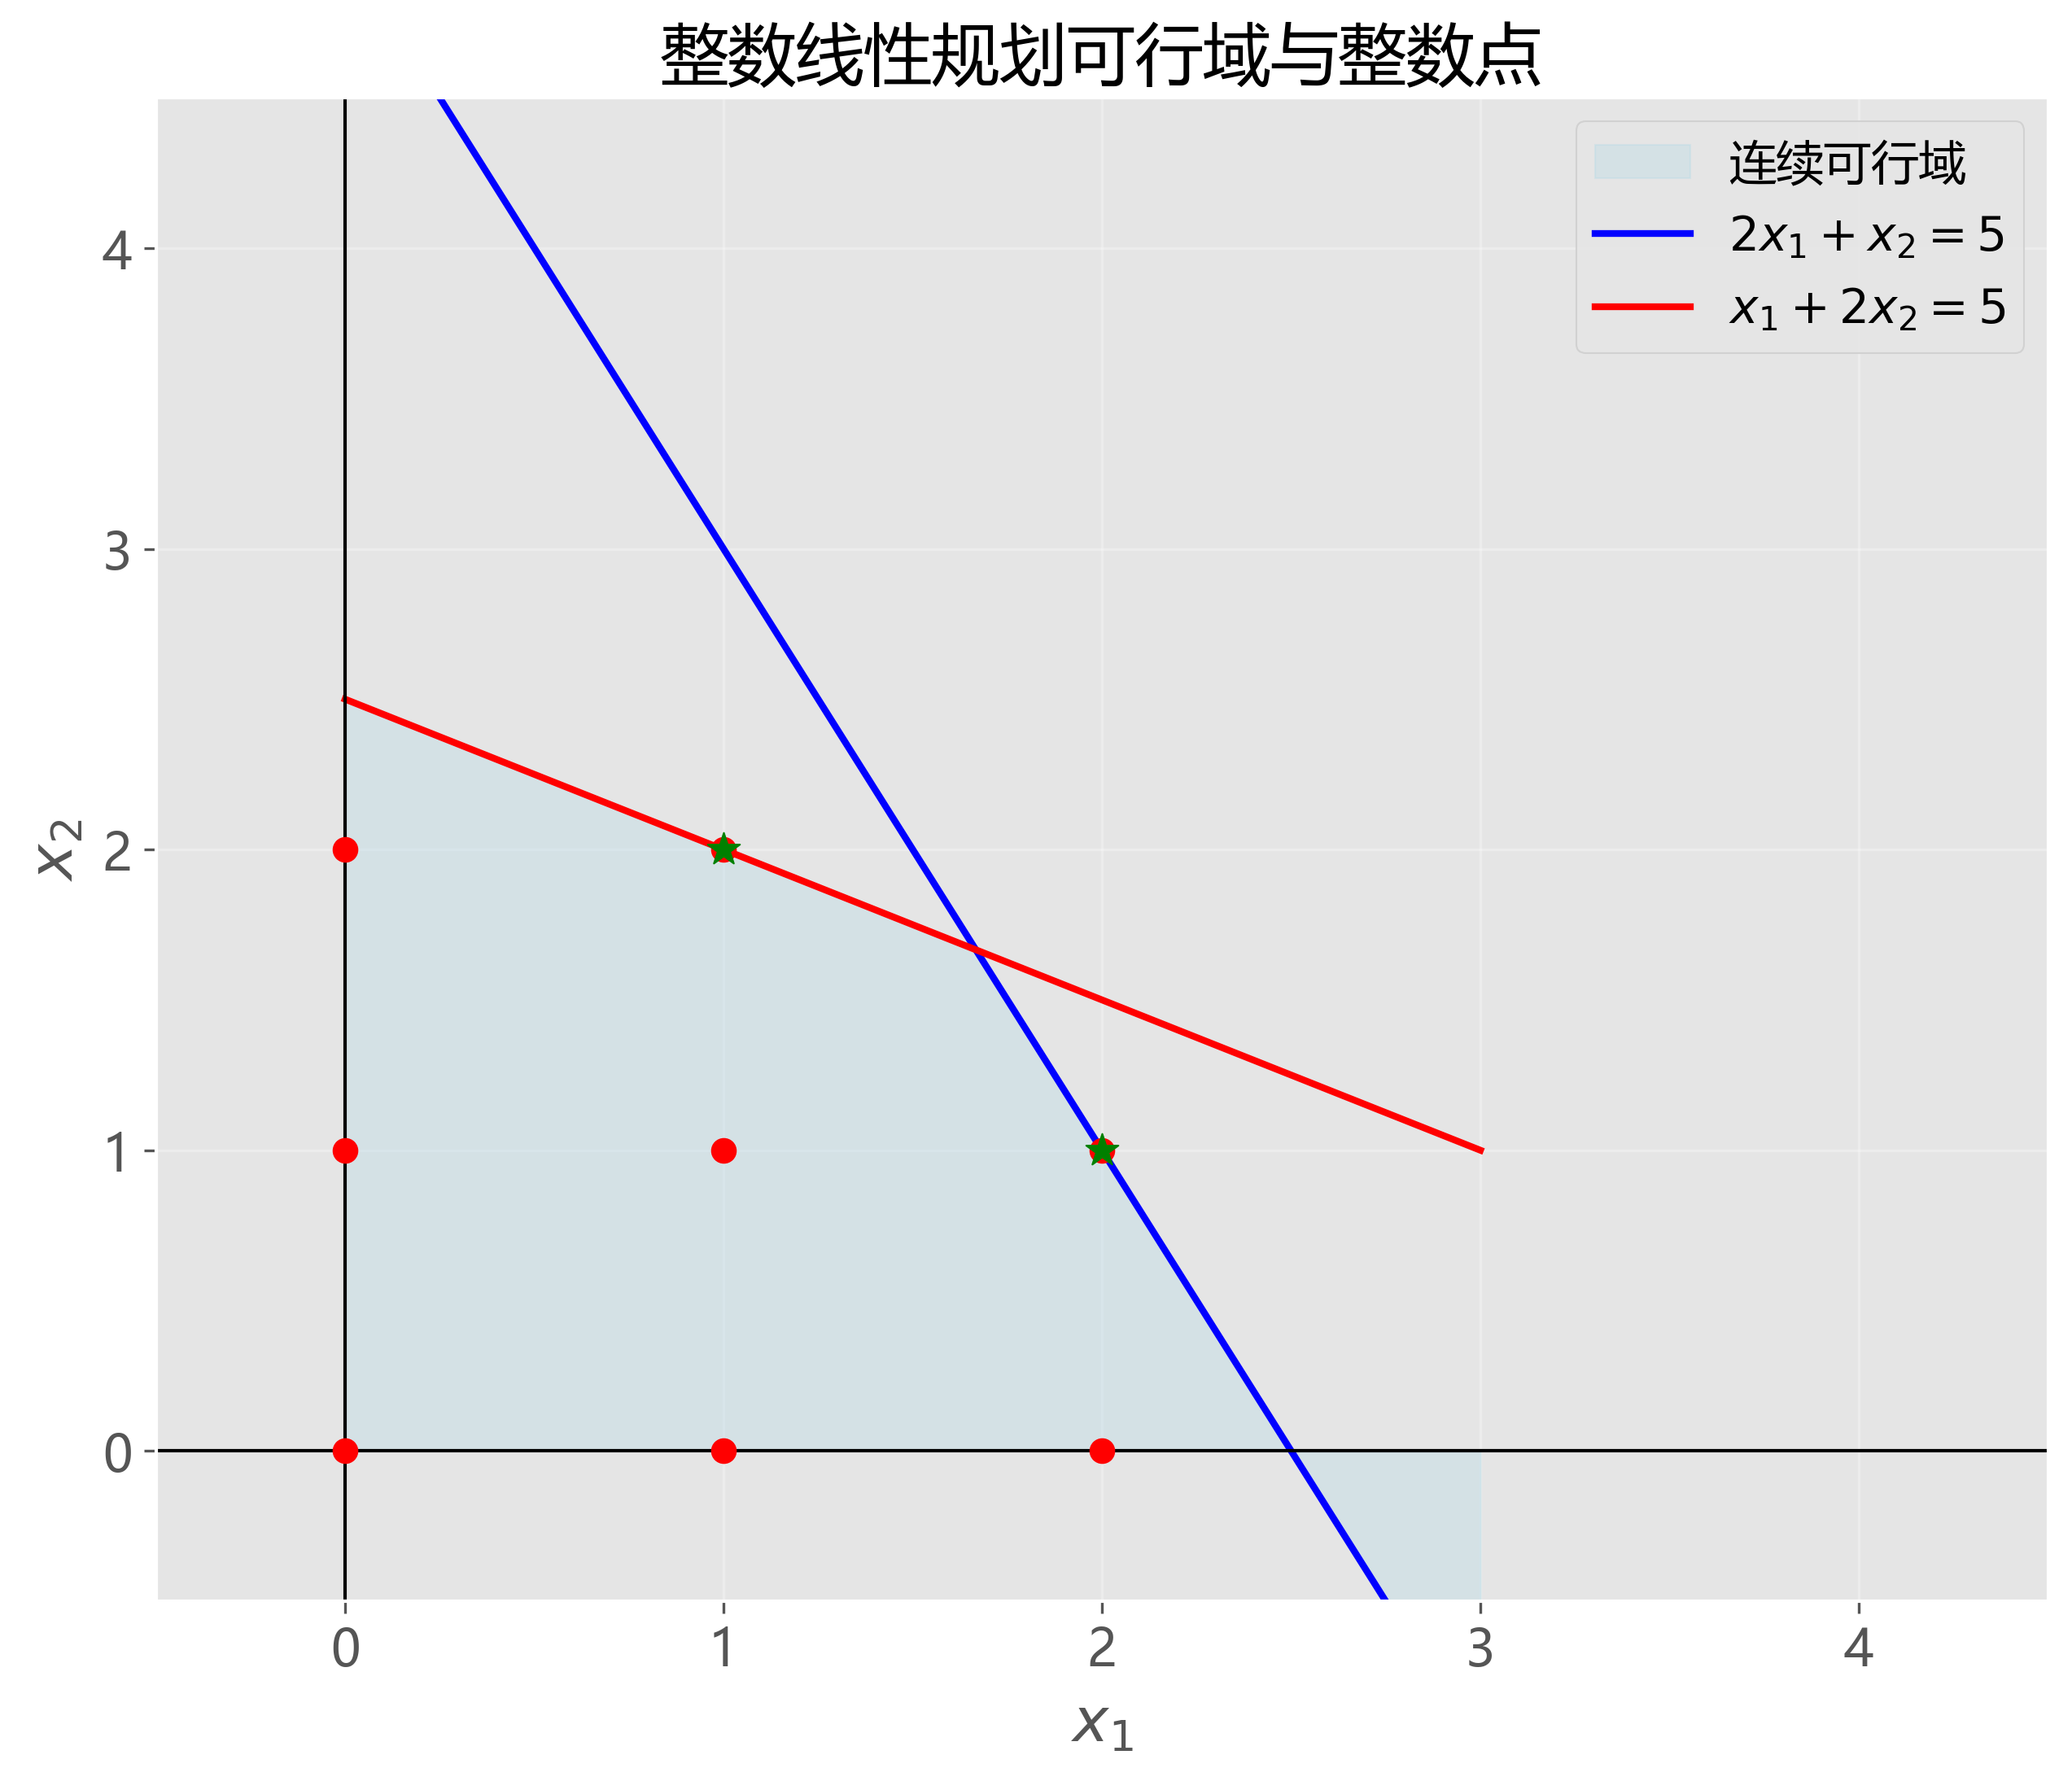
\includegraphics[width=0.8\textwidth]{integer_lp_plot.png}
        \caption{整数线性规划可行域与整数点}
        \label{fig:integer_lp}
    \end{figure}
\end{exm}
\begin{rmk}
    从图中可以看出，整数线性规划的可行域由离散的点组成。不同于线性规划的最优解一定在极点上，整数线性规划的最优解必须是满足约束的整数点，这些点可能位于连续可行域的内部或边界上：这带来了求解的复杂性。虽然在二维情况下我们可以通过图解来找到最优整数解，但在高维空间中，这种方法显然不可行，因此需要更系统的算法来处理整数规划问题。
\end{rmk}

\subsubsection{Gomory 割平面法}\label{subsubsec:gomory_cut}

割平面法（Cutting Plane Method）是一种求解整数线性规划的经典算法，最著名的变体是由 Ralph Gomory 提出的\textbf{Gomory 割平面法}。该方法的核心思想是：首先求解对应的线性规划松弛问题（即忽略整数约束），得到一个可能非整数的最优解；如果该解已经满足整数约束，则算法结束；否则，通过分析该非整数解，构造一个新的线性约束（割平面），将当前非整数解排除在可行域之外，同时保证所有满足整数约束的解仍然可行。重复这一过程，直到找到一个满足整数约束的最优解。

利用之前的图（图~\ref{fig:integer_lp}），我们可以直观地理解割平面法：如果我们得到的最优解是 $(\frac{5}{3}, \frac{5}{3})$，它不满足整数约束。我们可以通过分析该点与整数点之间的关系，构造一个割平面（例如 $x_1 + x_2 \leq 3$），将 $(\frac{5}{3}, \frac{5}{3})$ 排除在可行域之外，但仍然包含所有满足整数约束的点。就像在这些整数点外围上一圈“网”，不断收紧这个网，直到只剩下原可行域内最“外围”、且在先可行域内坐标均为整数的极点。针对这个例子，就需要添加 $x_1, x_2 \leq 2$ 和 $x_1 + x_2 \leq 3$ 三个割平面，才能将非整数解排除掉；当然，在算法设计中，只要找到一个最优点满足整数约束即可，不需要割去所有的非整数极点。那么，问题就转为如何求出割平面约束了。

\paragraph{割平面的数学推导}
考虑一个已用单纯形法求得最优解的线性规划松弛问题。设其最优单纯形表对应的约束方程为（用非基变量表示基变量）：
\[ x_{B_i} = \bar{b}_i - \sum_{j \in N} \bar{a}_{ij} x_j, \quad i = 1,\dots,m, \]
其中 $B_i$ 表示基变量下标，$N$ 为非基变量下标集，$\bar{b}_i$ 为当前基变量的取值，$\bar{a}_{ij}$ 为约束系数。所有变量（包括松弛变量）均非负。

若某个基变量 $x_{B_i}$ 的取值 $\bar{b}_i$ 不是整数，则当前的解不满足整数要求。我们希望添加一个线性不等式，使得：
\begin{itemize}
    \item 当前的非整数解被割掉（即不满足新不等式）；
    \item 所有整数可行解仍然满足新不等式。
\end{itemize}

将 $\bar{b}_i$ 和 $\bar{a}_{ij}$ 分解为整数部分和小数部分：
\[ \bar{b}_i = [\bar{b}_i] + f_i, \quad 0 < f_i < 1, \]
\[ \bar{a}_{ij} = [\bar{a}_{ij}] + f_{ij}, \quad 0 \le f_{ij} < 1. \]
其中 $[\cdot]$ 表示取不大于该数的最大整数。

将上述分解代入基变量表达式：
\[
x_{B_i} + \sum_{j \in N} [\bar{a}_{ij}] x_j = [\bar{b}_i] + \left( f_i - \sum_{j \in N} f_{ij} x_j \right).
\]
由于 $x_{B_i}$ 和 $[\bar{a}_{ij}] x_j$ 都是整数（变量取整数时，这些项的和为整数），因此等式左边为整数。从而右边也必须为整数，即括号内的表达式必须是整数：
\[ f_i - \sum_{j \in N} f_{ij} x_j \in \mathbb{Z}. \]
又因为 $0 < f_i < 1$ 且 $0 \le f_{ij} < 1$，$x_j \ge 0$，所以
\[ f_i - \sum_{j \in N} f_{ij} x_j \le f_i < 1. \]
要使它成为整数，只能取非正整数，即：
\[ f_i - \sum_{j \in N} f_{ij} x_j \le 0. \]
移项得 Gomory 割的一般形式：
\begin{equation} \label{eq:gomory_cut}
    \sum_{j \in N} f_{ij} x_j \ge f_i.
\end{equation}
将此不等式用原变量（包括松弛变量）表示，就得到了一个有效的割平面。

\paragraph{算法步骤}
\begin{enumerate}
    \item \textbf{初始化}：写出整数线性规划（ILP）的线性松弛问题（LP），并用单纯形法求解。
    \item \textbf{最优性检查}：若LP的最优解满足所有整数约束，则停止，该解即为ILP的最优解。
    \item \textbf{生成割平面}：从最优单纯形表中，选择一个取值非整数的基变量 $x_{B_i}$，按上述方法构造 Gomory 割：
        \[
        \sum_{j \in N} f_{ij} x_j \ge f_i,
        \]
        其中 $f_i$ 和 $f_{ij}$ 分别为常数和系数的小数部分。
    \item \textbf{添加割平面}：将割平面转化为等式约束（引入非负松弛变量），加入到当前LP中。
    \item \textbf{重新求解}：由于新约束使得原最优解不可行，但对偶可行性仍然保持（检验数非负），故采用\textbf{对偶单纯形法}求解新的LP。
    \item \textbf{重复}：转步骤2，直至找到整数最优解。
\end{enumerate}

\paragraph{一个完整的例子}
我们仍用之前的经典问题来说明 Gomory 割平面法的具体计算过程。
\begin{align*}
    \max \quad & z = x_1 + x_2 \\
    \st \quad & 2x_1 + x_2 \le 5 \quad (1)\\
    & x_1 + 2x_2 \le 5 \quad (2)\\
    & x_1, x_2 \ge 0, \quad x_1, x_2 \in \mathbb{Z}.
\end{align*}

\textbf{第1步：求解松弛问题}  
引入松弛变量 $x_3, x_4$，得标准型：
\begin{align*}
    \max \quad & z = x_1 + x_2 \\
    \st \quad & 2x_1 + x_2 + x_3 = 5 \\
    & x_1 + 2x_2 + x_4 = 5 \\
    & x_1, x_2, x_3, x_4 \ge 0.
\end{align*}
用单纯形法求解，初始表为：
\begin{table}[!htbp]
    \caption{初始表}
    \centering
    \begin{tabular}{c|cccc|c}
        \hline
        $z$ & $x_1$ & $x_2$ & $x_3$ & $x_4$ & \\ 
        \hline
        $z$ & -1 & -1 & 0 & 0 & 0 \\
        $x_3$ & 2 & 1 & 1 & 0 & 5 \\
        $x_4$ & 1 & 2 & 0 & 1 & 5 \\
        \hline
    \end{tabular}
\end{table}
经过两次转轴（先以 $x_2$ 入基、$x_4$ 出基，再以 $x_1$ 入基、$x_3$ 出基），得最优表：
\begin{table}[!htbp]
    \caption{最优表}
    \centering
    \begin{tabular}{c|cccc|c}
        \hline
        $z$ & $x_1$ & $x_2$ & $x_3$ & $x_4$ & \\ 
        \hline
        $z$ & 0 & 0 & $\frac{1}{3}$ & $\frac{1}{3}$ & $\frac{10}{3}$ \\
        $x_1$ & 1 & 0 & $\frac{2}{3}$ & $-\frac{1}{3}$ & $\frac{5}{3}$ \\
        $x_2$ & 0 & 1 & $-\frac{1}{3}$ & $\frac{2}{3}$ & $\frac{5}{3}$ \\
        \hline
    \end{tabular}    
\end{table}
最优解为 $x_1 = \frac{5}{3}, x_2 = \frac{5}{3}$，目标值 $z = \frac{10}{3}$，不是整数。

\textbf{第2步：构造 Gomory 割}  
选择基变量 $x_1$（取值 $\frac{5}{3}$），它对应的约束为：
\[ x_1 = \frac{5}{3} - \frac{2}{3}x_3 + \frac{1}{3}x_4. \]
将系数和常数分解为整数部分和小数部分（向下取整）：
\[
\frac{5}{3} = 1 + \frac{2}{3},\quad \frac{2}{3} = 0 + \frac{2}{3},\quad -\frac{1}{3} = -1 + \frac{2}{3}.
\]
代入原式：
\[
x_1 = 1 + \frac{2}{3} - \left(0 + \frac{2}{3}\right)x_3 + \left(-1 + \frac{2}{3}\right)x_4.
\]
移项，将所有整数项移至左边：
\[ x_1 + x_4 = 1 + \frac{2}{3} - \frac{2}{3}x_3 + \frac{2}{3}x_4. \]
整理得：
\[ x_1 + x_4 - 1 = \frac{2}{3}(1 - x_3 - x_4). \]
右边必须非负，因此：
\[ \frac{2}{3}(1 - x_3 - x_4) \ge 0 \quad \Longrightarrow \quad x_3 + x_4 \le 1. \]
或者按照割的一般形式：$\sum f_{ij}x_j \ge f_i$，此处非基变量为 $x_3, x_4$，它们的小数系数均为 $\frac{2}{3}$，常数小数部分 $f_i = \frac{2}{3}$，因此：
\[
\frac{2}{3}x_3 + \frac{2}{3}x_4 \ge \frac{2}{3} \quad \Longleftrightarrow \quad x_3 + x_4 \ge 1.
\]
两种形式等价（一个用 $\le$，一个用 $\ge$，取决于移项方向）。通常采用 $\ge$ 形式，因为它与对偶单纯形法兼容。我们取：
\[ x_3 + x_4 \ge 1. \]
回到原变量 $x_1, x_2$：由 $x_3 = 5 - 2x_1 - x_2$，$x_4 = 5 - x_1 - 2x_2$，代入得：
\[ (5 - 2x_1 - x_2) + (5 - x_1 - 2x_2) \ge 1 \quad \Longleftrightarrow \quad 10 -  3x_1 - 3x_2 \ge 1 \quad \Longleftrightarrow \quad x_1 + x_2 \le 3. \]
这就是 Gomory 割。

\textbf{第3步：添加割平面并重新求解}  
将 $x_1 + x_2 \le 3$ 加入原问题，引入松弛变量 $x_5$：
\[ x_1 + x_2 + x_5 = 3, \quad x_5 \ge 0. \]
此时问题变为：
\begin{align*}
    \max \quad & z = x_1 + x_2 \\
    \st \quad & 2x_1 + x_2 + x_3 = 5 \\
    & x_1 + 2x_2 + x_4 = 5 \\
    & x_1 + x_2 + x_5 = 3 \\
    & x_1, \dots, x_5 \ge 0.
\end{align*}
在最优表的基础上添加新行，并将当前基变量 $x_1, x_2$ 消去（使新行中只含非基变量），得：
\begin{table}[!htbp]
    \caption{添加割平面后的表}
    \centering
    \begin{tabular}{c|ccccc|c}
        \hline
        $z$ & $x_1$ & $x_2$ & $x_3$ & $x_4$ & $x_5$ & \\ 
        \hline
        $z$ & 0 & 0 & $\frac{1}{3}$ & $\frac{1}{3}$ & 0 & $\frac{10}{3}$ \\
        $x_1$ & 1 & 0 & $\frac{2}{3}$ & $-\frac{1}{3}$ & 0 & $\frac{5}{3}$ \\
        $x_2$ & 0 & 1 & $-\frac{1}{3}$ & $\frac{2}{3}$ & 0 & $\frac{5}{3}$ \\
        $x_5$ & 0 & 0 & -$\frac{1}{3}$ & -$\frac{1}{3}$ & 1 & -$\frac{1}{3}$ \\
        \hline
    \end{tabular}
\end{table}
此时 $x_5 = -\frac{1}{3} < 0$，且 $z$ 行检验数非负，满足对偶单纯形法的条件。选择 $x_5$ 出基，按最小比值原则选 $x_3$ 或 $x_4$ 入基（比值均为 $1$）。取 $x_3$ 入基，以 $-\frac{1}{3}$ 为主元进行转轴，得新表：
\begin{table}[!htbp]
    \caption{转轴后的表}
    \centering
    \begin{tabular}{c|ccccc|c}
        \hline
        $z$ & $x_1$ & $x_2$ & $x_3$ & $x_4$ & $x_5$ & \\ 
        \hline
        $z$ & 0 & 0 & 0 & $\frac{1}{3} + \frac{1}{3} \cdot \frac{1}{3}$ & $\frac{1}{3} \cdot \frac{1}{3}$ & $\frac{10}{3} + \frac{1}{3} \cdot \frac{1}{3}$ \\
        $x_1$ & 1 & 0 & 0 & $-\frac{1}{3} - \frac{2}{3} \cdot \frac{1}{3}$ & $\frac{2}{3} \cdot \frac{1}{3}$ & $\frac{5}{3} + \frac{2}{3} \cdot \frac{1}{3}$ \\
        $x_2$ & 0 & 1 & 0 & $\frac{2}{3} + \frac{1}{3} \cdot \frac{1}{3}$ & $-\frac{1}{3} \cdot \frac{1}{3}$ & $\frac{5}{3} - \frac{1}{3} \cdot \frac{1}{3}$ \\
        $x_5$ & 0 & 0 & 1 & $\frac{1}{3}$ & -$\frac{1}{3}$ & $\frac{1}{3}$ \\
        \hline
    \end{tabular}
\end{table}
得到新解：$x_1 = 1, x_2 = 2, x_3 = 1, x_4 = 0, x_5 = 0$，目标值 $z = 3$。所有基变量均为整数，且满足原约束，因此 $(x_1, x_2) = (1, 2)$ 是一个整数最优解（对称地，$(2,1)$ 也是最优解）。算法结束。

\paragraph{评注}
Gomory 割平面法的理论价值远大于其实用价值。虽然它可以在有限步内收敛，但实际计算中往往需要添加大量割平面，且数值稳定性较差。不过，它的思想深刻影响了后续的整数规划算法，成为割平面法的基石。现代商用求解器常将割平面法与分支定界法结合（称为“分支切割法”），以高效求解整数规划问题。

\newpage
\appendix
\section{单纯形法的C语言实现}\label{appendix:simplex_c_code}

以下是一个简单的单纯形法在C语言中的实现，用于求解标准形式的线性规划问题（最大化）。该实现假设矩阵为双精度浮点数，使用动态内存分配，并处理基本的转轴操作。注意：这是一个教学示例，未优化性能，且不处理所有边界情况（如退化、无界等）。


\end{document}




